\documentclass[11 pt]{scrartcl}
\usepackage[header, margin, koma]{tyler}
%\usetikzlibrary{automata,arrows,positioning,calc}
\usepackage{csquotes}

\pagestyle{fancy}
\fancyhf{}
\fancyhead[l]{CS 271 Notes}
\fancyhead[r]{Tyler Zhu}
\cfoot{\thepage}

\newcommand{\alg}{\mathcal{A}}
\newcommand{\Maj}{\text{Maj}}
\newcommand{\poly}{\text{poly}}
\newcommand{\satisf}{\text{ satisf.}}
\newcommand{\per}{\text{per}}
\newcommand{\EEm}{\EE_{\Acal_n}}
\newcommand{\PPm}{\PP_{\Acal_n}}


\begin{document} 
\title{\Large CS 271: Randomness and Computation}
\author{\large Tyler Zhu}
\date{\large\today}

\maketitle 

\begin{center}
\begin{displayquote}
    \emph{"A good stock of examples, as large as possible, is indispensable for a thorough understanding of any concept, and when I want to learn something new, I make it my first job to build one."} \\ \begin{flushright} \emph{– Paul Halmos}.  \end{flushright}
\end{displayquote}
\end{center}


These are course notes for the Spring 2020 rendition of CS 271, Randomness and Computation, taught by Professor Alistair Sinclair.

\tableofcontents 

\newpage

\section{Tuesday, January 21}

Instructors for this course are Alistair Sinclair (sinclair@cs), OH in 677 Soda Mondays 1-2PM and Thursday 11-12AM, and Kush Bhatia (kush@) in 347 Alcove Soda Tuesdays 2-3PM and Wednesday 10-11AM. 

Course website is at \texttt{https://people.eecs.berkeley.edu/\textasciitilde{}sinclair/cs271/s20.html}. There's no official textbook (but plenty of references); instead there is a set of fairly comprehensive lecture notes made available at the website.  

We will assume familiarity with undergraduate algorithms, complexity theory, and data structures. CS 170 is approximately enough. There will be roughly four homeworks (each will be somewhat meaty), so don't expect to leave it to the last minute. 

The philosophy of this class is to be more as a survey of techniques, rather than a deep dive into a specific topic. We'll look certain scenarios, and look at examples that use similar techniques. There will often be randomness (such as random graphs or random boolean circuits) because they sometimes serve as analogs for random inputs. Plus they're clean playgrounds for our purposes. 

We can also view randomness in complexity theory in relation to resources (such as saving or minimizing the number of random bits).  

\subsection{Introduction}
Typically we'll have an algorithm $\mathcal{A}$ which takes an input $x$ and outputs an answer $\mathcal{A}(x)$. We can tweak this by also generating (as part of the algorithm) as input some sequence of random bits $r$, so our output is now $\mathcal{A}(x, r)$, i.e. dependent on both deterministic and random values. As a result, this output is also a random variable, so we can ask questions such as $\PP[\mathcal{A}(x,r) = 0]$.
    Ideally this output isn't too far off from the true answer, otherwise this wouldn't be useful at all (just flip a coin). 

We can interpret this randomness as being generated from a Turing machine, where at each of $r$ timesteps we branch to choose either $0$ or $1$ as our bit, so there's $2^r$ possible outputs. While we can't exactly represent probabilities of say $\frac 13$ as a result, we can get arbitrarily close to it by approximation. In other words, all of our algorithms will have some errors associated with them. 

\subsection{Flavors of Randomized Algorithms}

Here's a brief list of some of the randomized algorithms we'll see: 
\begin{enumerate}
    \ii \textbf{Monte Carlo Algorithms}: Bounded error probability (output may be incorrect with small probability). These themsleves come in two flavors. 
    \alphanum
    \ii One-sided error: Yes answer is always right, but the No answer may sometimes be wrong. Formally, 
    \[ \text{ if true answer = ``yes'' }\implies \PP[\alg\text{ outputs ``yes''}] \geq \eps > 0 \]
    \[ \text{ if true answer = ``no'' }\implies \PP[\alg\text{ outputs ``no''}] = 1.\]

    This looks really bad, because in one case we have a guaranteed answer, but in the other case we have only an $\eps$ probability of being correct. In other words, probability of error (one-sided) is $\leq 1-\eps$. But say we perform this test $t$ times independently, and output ``yes'' if any trial outputs ``yes'', else output ``no''. Then 
    \[ \PP[\text{error}] \leq (1-\eps)^t \leq \delta\] 
    if we take $t = O(\log 1/\delta)$ for your favorite choice of $\delta$. The class of decision problems for which there exist one-sided error algorithms that run in polynomial time is RP, i.e. ``randomized polynomial time.'' If the yes and no decisions are flipped, then the class becomes co-RP. 

    \ii Two-sided errors:  
    \[ \text{ if true answer = ``yes'' }\implies \PP[\alg\text{ outputs ``yes''}] \geq \frac{1}{2} + \eps \]
    \[ \text{ if true answer = ``no'' }\implies \PP[\alg\text{ outputs ``yes''}] \leq \frac{1}{2} - \eps .\]
    
    We need the epsilon here because we can do a similar trick from the above in order to concentrate the probability and make it stronger. Repeat $t$ times and take a majority vote. One can use Chernoff/Hoeffding bounds to see this in general, but here we can do it from first principles. 

    In order to make a wrong decision, we need a majority of the outputs to be incorrect, so 
    \begin{align*}
        \PP[\text{error in }t\text{ trials}] &= \PP[\text{obtain } \leq \frac{t}{2}\text{ correct outputs}] \\ 
                                             &\leq \sum_{i=0}^{\floor{t/2}} \dbinom{t}{i} (\frac{1}{2} + \eps)^i (\frac{1}{2}-\eps)^{t-i} \\ 
                                             &\leq \sum_{i=0}^{\floor{t/2}} \dbinom{t}{i} (\frac{1}{2} + \eps)^{t/2} (\frac{1}{2}-\eps)^{t/2} \\ 
                                             &= (\frac{1}{4} - \eps^2) ^ t \sum_{i=0}^{\floor{t/2}} \dbinom{t}{i} \leq (1-4\eps^2)^{t/2} \\ 
                                             &= \delta
    \end{align*}
    if we take $t = O(\log \delta^{-1})$. We refer to the class of decision problems that have a 2-sided error randomized algorithm in polynomial time as \textbf{BPP}.
    \enumend

    \ii \textbf{Las Vegas Algorithms}: Output is always correct, and the \emph{expected} running time is bounded. Equivalently, the running time is bounded and the output is always correct, but the algorithm may output ``?'' with probability $\leq 1/2$. 
    \begin{exercise}
    Check that these are equivalent formulations.
    \end{exercise}
    \begin{proof}
        Say the expected running time is $t$. Then run it for $2t$ steps, and by Markov's inequality, the probability it hasn't completed is $1/2$. Conversely, if we have the latter scenario, then with probability 1 it completes running. Say it has probability $1/2$ of outputting an answer by time $t$: then the overall time is $\frac{1}{2}t + \frac{1}{4}(2t) + \dots$ which coverges to $t$.  
    \end{proof}

    The class of decision problems with a Las Vegas algorithm with polynomial bounded expected running time is \textbf{ZPP}, i.e. zero-error polynomial time. 
\end{enumerate}

We can draw a picture of these complexity classes. We would draw RP and co-RP, and ZPP would lie somewhere in the middle. In fact, ZPP is \emph{exactly} the intersection between these two classes. 

\begin{exercise}
    Prove that ZPP = RP $\cap$ co-RP. 
\end{exercise}

BPP contains everything (and more), while P would be inside ZPP and NP would contain RP and some of BPP.

\begin{figure}[!htb]
    \centering
    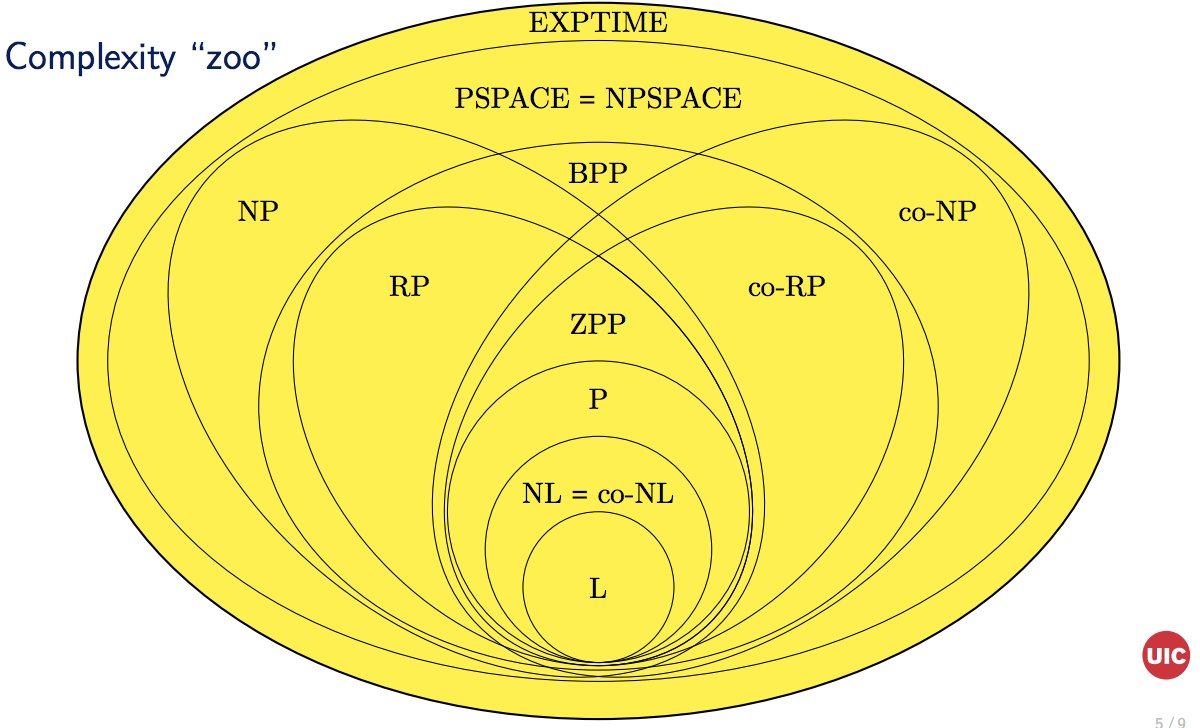
\includegraphics[scale=0.3]{complexity.jpg}
    \caption{The big picture.}
\end{figure}

The open questions in this field are if P = RP and if P = BPP; in otherwords, we want to know if randomness buys you anything. 

\begin{itemize}
    \ii If P = BPP, then we don't gain much from randomness, but it would not imply P = NP. 
    \ii If P = NP, then everything collapses (including BPP). This follows from a result in compelexity classes, where it's known that BPP $\subseteq$ $\text{NP}^{\text{NP}}$ (the second order of NP). In this case, $\text{NP}^{\text{NP}}$ = P.  
    \ii If $NP \subseteq BPP$, then $NP$ has polynomial size classes (very unlikely). 
\end{itemize}

Here's a remarkable theorem which, out of two things we'd both like to be true, states that one of them must be false. 
\begin{theorem}[Impagliazzo-Wigderson]
    If SAT cannot be solved by circuits of size $2^{o(n)}$, then BPP = P. 
\end{theorem}
In other words, if what we believe about NP algorithms is true (i.e. we should need exponentially amount of work to solve SAT), then randomness doesn't actually buy you anything. But if it turns out randomness does help, then there exist sub-exponential sized circuits to solve SAT. Both are remarkable statements. 

This also doesn't imply that P = NP quite yet, as there's some tricky point about how your circuits grow with your inputs, but that's a problem for another class. 

Here's another philosophical question. Suppose we do show that randomness does help. We still have the following problem: say you're implementing a randomized algorithm. Where do you get your random bits? Random number generators are usually pseudo-random, i.e. are pregenerated, but we also can't tell the difference between truly random algorithms and pseudo-random ones. If BPP is different from P, then we wouldn't be able to simulate algorithms that express this difference. We would need a source of true randomness. 


Most complexity theorists bet that BPP = P, and even though conceptually these algorithms are most clean, there are most likely going to be huge overheads that would make them infeasible to use realistically. 

\subsection{Examples of Randomized Algorithms: Matrix Multiplication, Associativity}

In the following examples, we want to be able to check if the answer is correct without having to do the same amount of work as the computer did. Philosophically, checking should be easier than doing. With the help of randomness, we can do this.  
\begin{example}[Check Matrix Multiplication]
    Suppose we have as input three $n\times n$ matrices $A,B,C$. 
    \begin{question}
        Is $AB = C$? 
    \end{question}
    Algorithm: Pick a random vector $(r_1, r_2, \dots, r_n)$ such that each $r_i$ is chosen independentaly and uniformly at random from a set $S$, $|S| \geq 2$. If $A(Br) \not= Cr$, then output ``no'', else output yes. This is faster, i.e. $O(n^2)$, as we're only doing matrix-vector multiplication (unless matrix multiplication achieves $O(n^2)$ time). 

    This is an example of what we call a \emph{Witness search}, as we're searching for a vector which is a witness that $AB \not= C$. Clearly this is a one-bounded algorithm. 

    Claim: If $AB \not= C$, then $\PP[(AB)r = Cr] \leq \frac{1}{|S|}$. 
    \begin{proof}
        Define $D = AB - C$. Suppose $D \not= 0$, and WLOG $d_{11} \not= 0$, i.e. the upper-left corner is not 0. 

        Let's look at the first vector of $D$. We know that 
        \begin{align*}
            (Dr)_1 &= \sum_{i = 1}^n d_{1i}r_i = 0 \\ 
            r_1 &= -\frac{1}{d_{11}} \sum_{i = 2}^n  d_{1i} r_i
        \end{align*}
        So the probability that $r_1$ is the one number that makes this entire sum 0 is $\leq \frac{1}{|S|} \leq \frac{1}{2}$. 
    \end{proof}
\end{example}

\begin{example}[Testing Associativity (Rajagoparlan/Schulman)]
    Suppose we have as input a binary operator $\circ$ on a set $X$ of size $n$. 
    \begin{question}
        Is $\circ$ associative, i.e. $(i\circ j)\circ k = i \circ (j\circ k)$ for $i,j,k \in X$? 
    \end{question}
    One naive idea is to just test triples for associativity, but it turns out there exist binary operators which are mostly associative except for sometimes a \emph{constant} amount of witnesses. Instead, the key idea will be to test subsets. 

    Algorithm: Consider \emph{sets} of elements $R, S, T \in 2^X$. 
    Pick $R, S, T$ independently and u.a.r. over $2^X$. If $(R\circ S)\circ T \not= R\circ (S\circ T)$, then output ``no'', else output ``yes''. 

    This works because of the following fact:
    \begin{exercise}
        Check that $\circ$ is associative over $X$ iff $R\circ(S\circ T) = (R\circ S)\circ T \;\;\forall R,S,T \in 2^X$. 
    \end{exercise}


    We can do this check in $O(n^2)$ (for all members of the subset) using vector dot products (think of elements as tuple $(r_i, i)$ where $r_i$ is 1 if $i\in R$, and 0 else). In this case, we can create a giant lookup table of products and reference from there, so computing products is constant time and creating this table is $O(n^2)$. This is faster than the $O(n^3)$ needed to check all triples of $X$. 

    The heart of the algorithm is the following claim, which is a clever application of the principle of inclusion-exclusion. 
    
    \begin{claim}
        If $\circ$ is not associative, then at least $1/8$ of the tuples $(R, S, T)$ are witnesses. 
    \end{claim}
    \begin{proof}
        Partition $2^X$ into disjoint groups of 8. Assume $\circ$ is not associative, so there exists $i^*, j^8, k^* \in X$ such that $(i^*\circ j^*)\circ k^* = i^* \circ(j^* \circ k^*)$. 

        Let $R_0, S_0, T_0$ be any subsets s.t. $i^*, j^*, k^* \not\in R_0, S_0, T_0$. Let $R_1 = R_0 \cup \{i^*\}$, $S_1 = S_0 \cup \{j^*\}$, $T_1 = T_0 \cup \{k^*\}$. Now we have 8 triples $\{(R_a, S_a, T_a) | a \in \{0,1\}\}$. Define $f(R, S, T) = |(R\circ S)\circ T - R\circ (S\circ T)|$, i.e. the number of witnesses in each triplet of sets. Then by inclusion-exclusion, we can write 
        \begin{align*}
            f(i^*, j^*, k^*) &= f(R_1, S_1, T_1) \\ 
                             &- f(R_0, S_1, T_1) - f(R_1, S_0, T_1) - f(R_1, S_1, T_0) \\ 
                             &+ f(R_0, S_0, T_1) + f(R_0, S_1, T_0) + f(R_1, S_0, T_0) \\ 
                             &- f(R_0, S_0, T_0).
        \end{align*}
        Since we know that the LHS is nonzero, at least one of the terms on the right has to be nonzero as well, from which our claim follows. 
    \end{proof}

\end{example}

\newpage
\section{Thursday, January 23rd}
\subsection{More Randomized Algorithms: PIT, Perfect Matchings}
\begin{example}[Polynomial Identity Testing]
    Suppose we have as input a polynomial $Q(x_1, \dots, x_n)$. 

    \begin{question}
        Is $Q = 0$? 
    \end{question}
    To understand the motivation for this, suppose we wanted to ask if $(x_1+x_2)(x_1-x_2) = x_1^2 - x_2^2$. Then we could make $Q(x_1, x_2)$ the difference of the two polynomials to test for equality. 

    For a more complicated example, consider the Vandermonde determinant 

    \[ \det \begin{pmatrix} 1 & 1 & \dots & 1 \\ 
                            x_1 & x_2 & \dots & x_n \\ 
                            \vdots & \vdots & \vdots & \vdots \\ 
                            x_1^{n-1} & x_2^{n-1} & \dots & x_n^{n-1} \end{pmatrix}
                        = \prod_{i<j} (x_j-x_i).\] 

    It's very nontrivial to see if these two polynomials are the same. 

    Algorithm (Schwartz-Zippel): Pick a random point $(r_1, \dots, r_n)$ where each $r_i$ is chosen u.a.r. from a set $S$. Test if $Q(r_1, \dots, r_n) = 0$. 

    \begin{claim}
        If $Q(x_1, \dots, x_n)$ is a non-zero polynomial of degree $d$, then $\PP[Q(r_1, \dots, r_n) = 0] \leq d/|S|$. 
    \end{claim}

    \begin{proof}
        Induction on the number of variables $n$. 

        Base case: $n=1$, which is the univariate case and follows from the Fundamental Theorem of Algebra.  

        Inductive step: Write 
        \[ Q(x_1, \dots, x_n) = A(x_2, \dots, x_n)x_1^k + B(x_1, \dots, x_n).\]
        Assume $k$ is the largest power of $x_1$, so that $\deg(A) \leq d-k$ and degree of $x_1$ in $B$ is $< k$. 
        
        Assume $x_2 = r_2, \dots, x_n = r_n$ are chosen first. Let $\mathcal{E}$ be the event that $A(r_2, \dots, r_n) = 0$. We have two cases: 
        \alphanum
            \ii $\mathcal{E}$ happens, which by induction has probability $\PP[\mathcal{E}]\leq (d-k. )/|S|$. 
            \ii $\mathcal{E}$ doesn't happen. So $A(\cdot)x_1^k + B(\cdot)$ is a non-zero univariate polynomial in $x_1$. Also, since $\deg B < k$ (as we pulled out the highest powers into $A$), $\PP[Q(r_1, \cdots, r_n) = 0 | \neg \mathcal{E}] \leq k/|S|$ by base case.  
        \enumend
        Summing them up, we have that

        \[ \PP[Q = 0] = \PP[Q = 0 | \mathcal{E}]\PP[\mathcal{E}] + \PP[Q = 0 | \neg \mathcal{E}]\PP[\neg\mathcal{E}] \leq \dfrac{d-k}{|S|} + \dfrac{k}{|S|} = \dfrac{d}{|S|}.\] 
    \end{proof}

\end{example}

    This is a remarkable algorithm because it convinced people that randomness is useful. Without randomness, we have no clue how to approach this problem.   

\begin{question}
    Can this algorithm be derandomized? 
\end{question}
\begin{theorem}[Impagliazzo-?]
    If PIT can be solved determinstically in poly time then either 
    \begin{enumerate}[(1)]
        \ii The permanent\footnote{The \emph{permanent} is the determinant but without the $\text{sgn}(\si)$ factor in the expansion; see later in this section.} cannot be computed by poly size circuits, OR
        \ii NEXP does not have poly size circuits.  
    \end{enumerate}
\end{theorem}

Recall that a \emph{matching} in a bipartite graph $\mathcal{G} = (V_1, V_2, E)$ is a collection of edges so that no vertex is in more than one edge in that collection. A \emph{perfect matching} is a matching which contains every single vertex. 

Recall that there are algorithms to determine if a graph has a perfect matching (and to find one), such as Edmonds-Karp flow based algorithm. But none are very efficient, so instead we'll develop a randomized one. 

\begin{example}[Perfect Matchings]
    Suppose we have a bipartite graph $\mathcal{G} = (V_1, V_2, E)$ as input. 

    \begin{question}
        Does there exist a perfect matching in $\mathcal{G}$?
    \end{question}
    
    Given $\mathcal{G}$, construct the \emph{Tutte matrix} $A_\mathcal{G}$ which is an $|V_1|\times|V_2|$ matrix where the indeterminate $x_{ij}$ is in the $ij$-entry if there is an edge from $i\in V_1$ to $j\in V_2$ and zero otherwise. 

    \begin{claim}
        $\mathcal{G}$ has a perfect matching iff $\det(A_\mathcal{G}) \not= 0$. 
    \end{claim}
    \begin{proof}
        We expand the determinant as 
        \[ \det(A_{\mathcal{G}}) = \sum_{\si\in S_n} \text{sgn}(\si) \prod_{i=1}^n a_{i\si(i)}.\] 
        Now apply the Schwartz-Zippel algorithm to test if $\det(A_{\mathcal{G}}) \not= 0$ as a polynomial. The degree is $n$ so we need to plug in random values distributed uniformly in $\{1, 2, \dots, 2n\}$. 
    \end{proof}
\end{example}

We can also extend this result to general graphs (not just bipartite)
\begin{example}[Perfect Matchings for general graphs]
    Instead of using the Tutte matrix, we'd use the skew-symmetrix matrix 

    \[ B_{\mathcal{G}} = \begin{pmatrix} 0 & & & \\ 
                                          & \ddots & -x_{ij} & & \\ 
                                            & x_{ij} & \ddots & \\ 
                                            &   & & 0 \end{pmatrix}.\] 
        We can make the same claim here, which is that $\det(B_{\mathcal{G}}) \not= 0$ iff $\mathcal{G}$ has a perfect matching. 
\end{example}

\subsection{Parallelizing Algorithms}

We can efficiently parallelize such algorithms. There's a complexity class called NC where we can solve problems in $\text{polylog}(n)$ time and $\text{poly}(n)$ processors, and it's a fact that computing determinants is in NC. As an aside, NC$\subseteq$P. 

There's a naive idea for parallelizing this decision problem to determine perfect matchings. Remove an edge, run the algorithm, and recursively run until we determine edges that must be in the perfect matchings and repeat. 

This is parallelizable across choices of edges, but the subprocesses can't be run in parallel. One pitfall however is that not only are we doing work in cases multiple times, but that we may have \emph{multiple} perfect matchings, so our processes may be working on different matchings on the same time. If we want only one matching, then this is a waste of effort! 

There's a lemma to help us with this however, due to Mulmanley/Vazirani/Vazirani (both the professor at Berkeley \emph{and} his brother).  

\begin{lemma}[Isolation Lemma]
    Let $S_1, \dots, S_k$ be arbitrary subsets of a set $S$ of cardinality $m$. Let each element $x\in S$ have a weight $w_x$ chosen independently and u.a.r.  from $\{1, \dots, l\}$. Then 
    \[ \PP[ \exists\text{ unique min. weight set }S_i] \geq \left(1-\frac{1}{l}\right)^m \geq 1 - \dfrac{m}{l}.\] 
\end{lemma}

This is enough for our purposes of randomization as long as we take $l = 2m$ approximately so that the probability is greater than 1/2. The proof is due to a high school student in Israel. \footnote{What were you doing when you were in high school?}

\begin{proof}[Proof due to Ta-Shma]
    Assume w.l.o.g. that $S_i \not\subseteq S_j$ for any $i,j$. Let $\mathcal{W}$ denote the set of all weight functions $\{w_x\}$, and $\mathcal{W}^+$ denote the set of all weight functions such that $w_x > 1$ for all $x\in S$. The proof rests on the following claim.

    \begin{claim}
        For each function $w\in \mathcal{W}^+$, we can associate a \emph{distinct} function $w'\in \mathcal{W}$ such that $w'$ has a unique minimum weight set. This implies 
        \[ \PP[\exists\text{ unique minimum weight set}] \geq \dfrac{|\mathcal{W}^+|}{|\mathcal{W}|} = \left(1-\dfrac{1}{l}\right)^m \] 
        as we claimed above. 
    \end{claim}
        We prove the claim as follows. Take a function $w\in \mathcal{W}$ - pick \emph{any} minimum weight set $S_i$ under $w$. Construct $w'$ via 
        \[ w'_x = \begin{cases} w_x-1 \quad \text{ if } x \in S_i \\ w_x \quad \text{ otherwise} \end{cases}.\] 
        Then $w'$ has unique minimum weight set and can recover $w$ from $w'$. 
\end{proof}

Using this, we can create an algorithm for finding a perfect matching in a bipartite graph in parallel. 
\alphanum
    \ii Set each edge weight $w_{ij}$ as in the Isolation Lemma (with $S = E, l \geq 2|E|$). 
    \ii By the Isolation Lemma, $\mathcal{G}$ has min. weight. perfect matching with probability $\geq 1/2$.
    \ii Plug into Tutte matrix the values $2^{w_{ij}}$ (rather than $x_{ij}$) - call this matrix $A$. 
    \begin{itemize}
        \ii Calculate $2^w$, the largest power of 2 that divides $\det(A)$, which really looks like $\sum_M (\pm 1) 2^{w(M)}$. 
        \ii For each edge $(i,j)$ in parallel: 
            \begin{enumerate}[-]
                \ii compute $t_{ij} = 2^{w_{ij}}\det(A_{ij})$ where $A_{ij} = \{i,j\} - \text{ minor of }A$. 
                \ii include $(i,j)$ in perfect matching iff largest power of 2 that divides $t_{ij}$ is $2^w$.
            \end{enumerate}
        \ii Check that the selected edges from a perfect matching and output it if so. 
    \end{itemize}
\enumend

There's a ``quasi-parallel'' algorithm due to Svensson and Tarnaski for perfect matchings in polylog time and $n^{\text{poly}\log(n)}$ processors by derandomizing the Isolation Lemma by exploiting structure in perfect matchings. Anan Nazirani also has an NC algorithm for planar graphs. 

\newpage
\section{Tuesday, January 28th}
We'll talk a lot about primes today, including applications to testing equality of numbers and primality testing. 

\subsection{Fingerprinting}
\begin{example}[Testing Equality of Large Numbers]
Alice and Bob are on different planets, and they each of a large piece of data. They want to test if their data is the same. Let their data be $n$-bit numbers $a$ and $b$ respectively where $n$ is \emph{very} large. We want to test if $a = b$. 

Of course Alice could send $a$ to Bob, but this is probably prohibitively expensive. What we'll show instead is that Alice will send a fingerprint to Bob, and Bob will determine (w.h.p.) is $b$ is equal to $a$ based on that. 

Algorithm: Alice picks a random prime $p \in \{1,2,\dots, T\}$ (for a small $T$) and computes a fingerprint $F_p(a) = a\mod p$ and sends both $F_p(a)$ and $p$. Bob then computes his fingerprint, and if $F_p(a) = F_p(b)$ he responds Yes, otherwise he responds No. 

Note that this is a one-sided error: if $a = b$, then Bob will always respond Yes, and otherwise he responds No with some probability based on the $T$ we pick. We will analyze this latter case. 

Suppose $a\not= b$ and $F_p(a) = F_p(b)$. Then $p | (a-b)$ (where $a-b$ is an $n$-bit number). Crudely, the number of primes dividing $a-b$ is at most $n$ (as $\log(a-b)$ is a good lower bound). Now we make use of the following classical fact:

\begin{theorem}[Prime Number Theorem]
    Define $\pi(x) = \text{\# of primes }\leq x$ to be the prime counting function. Then, 
    \[ \dfrac{x}{\ln x} \leq \pi(x) \leq 1.26 \dfrac{x}{\ln x} \quad \forall\, x \geq 17.\] 
\end{theorem}

Thus, we can compute 
\[ [\text{\# of primes} \leq T] \approx \dfrac{T}{\ln T}\]
and thus 
\[ \PP[\text{error}] \leq \dfrac{n\ln T}{T}.\] 

So we should take $T = cn$ so that $\PP[\text{error}] = \frac{1}{c} + o(1)$. 

In fact, we can make a much more refined upper bound by using $\pi(x)$ an an upper bound on the number of primes that divide $a-b$. This gives 
\[ \PP[\text{error}] \leq \pi(n) \dfrac{\ln T}{T} \leq 1.26 \dfrac{n}{\ln n}\dfrac{\ln T}{T}.\] 
\end{example}
The hard part of this example then is to pick a random prime $p$. The PNT guarantees that the density of primes is quite decent in this range, and we'll look at algorithms for testing primality later in today's lecture, so Alice can just keep trying random numbers. 

\begin{example}[Pattern Matching]
    Suppose we have a source text $X = x_1x_2\dots x_n$ and a pattern $Y = y_1y_2\dots y_m$, $m < n$. We want to determine if $Y$ occurs in $X$. 

    There's an obvious $O(mn)$ brute force algorithm, but there's also some classical results in algorithms such as Boyer/Monse or Knuth/Morris/Pratt that solve this in $O(m + n)$. There is also a nice randomized algorithm in $O(m+n)$ found by Rabin/Karp. The main idea is to maintain a sliding window and compare finger prints of $X$ to the fingerprint of $Y$. 

    \textbf{Algorithm}: Pick a random prime $p \in \{1, 2, \dots, T\}$. Compute $F_p(Y) = Y \mod p$. Then, for $j = 1$ to $n-m+1$:
    \begin{itemize}
        \ii compute $F_p(X_j)$
        \ii if $F_p(X_j) = F_p(Y)$ output ``match'' and halt.  
    \end{itemize}
    otherwise output ``no match.''

    How big should $T$ be? We just use our previously calculated bound so that 
    \[ \PP[\text{error}] \leq n \dfrac{\pi(m)}{\pi(T)}.\] 
    We can do better though. For $p$ to be \emph{bad}, it must divide one of the $Y-X_j$'s, so it also divides 
    \[ \prod_{j=1}^{n-m+1} (Y-X_j) \leq nm\text{ bits },\] 
    so it suffices to take $T = cnm$ which gives a $O(\log n)$ bit fingerprint. 
\end{example}

One issue is how we would compute each of the $X_j$'s efficiently. Using our sliding window trick, we can compute each next $X_{j+1}$ based on the previous one efficiently since 
\[ X_{j+1} = 2(X_j - 2^{n-1}x_j) + x_{j + m}\] 
so 
\[ F_p(X_{j+1}) = 2(F_p(X_j) - 2^{n-1}x_j) + x_{j+m}.\]
Updating our fingerprints only takes $O(1)$ time then. 

\subsection{Primality Testing}

\begin{example}[Primality Testing]
    We have an integer $n$ as input (potentially hundreds or thousands of bits), and we want to determine if $n$ is prime. 
    
    You might try a prime number sieve, but those are typically polynomial in $n$, which is infeasible for our purposes. Another idea is to test divisors, but large numbers typically have very few divisors, so this will be inefficient. 

    One good idea is to start with Fermat's Little Theorem, which is the following: 
    \begin{theorem}
        If $p$ is prime then $a^{p-1} \equiv 1$ for all $a \in \{1, 2, \dots, p-1\}$.
    \end{theorem}
    Using this, we can pick a random number $a$ and see if $a^{p-1} \equiv 1$. If this is true, then we output prime, and otherwise we output not prime. This is called the \emph{Fermat test} and is actually used in practice. 

    Unfortunately, there are numbers for which $a^{p-1}\equiv 1$ yet are not primes; these are known as the Carmichael numbers, and we'll talk about them later. 

    A better insight is the following:
    \begin{fact}
        Suppose $n$ is not prime and not \emph{all} $a$'s satisfy $a^{n-1} \equiv 1 \mod n$. Then $\PP[\text{error}] \leq 1/2$. 
    \end{fact}
    This is because the group of witnesses is a subgroup of the multiplicative group $Z_n^\times$ on $n$ number (multiplicative group of integers $\mod n$ s.t. $\gcd(a,n) = 1$), so we can apply Lagrange's Theorem. 

    Let $S_n = \{a\in \ZZ^\times \text{ s.t. } a^{n-1}\equiv 1 \mod n\}$. Then this is a proper subgroup if $S_n \not\cong \ZZ^\times$ (which happens if $n$ is a Carmichael number), and its order cannot be more than half of that of $\ZZ^\times$. This is also the set of all witnesses, so our result follows.  

    To do better, we need a better witness test to weed out Carmichael numbers. 
    \begin{theorem}[Miller/Rabin Primality Test]
        Witnesses to compositeness of $n$ are non-trivial square roots $p$. Suppose $p$ is prime. Then there exists exactly two solutions to $x^2-1$ in $\ZZ_p$. If we can find a number $a$ s.t. $a^2 \equiv 1 $, $a\not= \pm 1$ in $\ZZ^\times$ then $n$ is not prime. 
    \end{theorem}
    For example, if $n = 7,8$, then try $a = 7$.  

    If $n = 2$ is even or a perfect power then output composite. Otherwise, compute $r,p$ such that $n - 1 = 2^{r}p$ (where $p$ is odd). 

    Then pick $a \in \{1, \dots, n-1\}$ u.a.r. If $\gcd(a,n) \not= 1$, then output composite. Otherwise, compute $b_i = a^{2^i p}$ for $i = 0, 1, \dots, r$ so that this sequence is 
    \[a^p, a^{2p}, \dots, a^{2^r p} = a^{n-1}.\]

    If $b_r \not= 1$ then output composite. Otherwise, if $b_0 = 1$ then output ``prime?''. Otherwise, let $j = \max\{i : b_i \not= 1\}$. If $b_j \not= -1$ then output composite, otherwise output ``prime?''. One should try this when $n = 561$ and $a =2 $. 

    \begin{claim}
        If $n$ is composite, odd, and not a prime power, then $\PP[a\text{ is not a witness}] \leq 1/2$. 
    \end{claim}
    \begin{proof}
        Show that non-witnesses lie in a proper subgroup by using Lagrange's theorem. 

        Say that $s$ is a \emph{bad power} if $x^s \equiv \pm 1 \mod n$ for some $x \in \ZZ^\times_n$. We claim that 
        \[ H_s = \{x \in \ZZ_n^\times | x^s = \pm 1 \mod n\}\] 
        is a proper subgroup of $\ZZ_n^\times$ for any bad power $s$. 

    Before we prove this claim, let's see how we'd finish with it. Apply this claim to $H_{s^*}$ where $s^*$ is the largest bad power. Suppose $a$ is a non-witness. Then either 
    \[ a^r = a^{2r} = \dots = a^{n-1} = 1\mod n\]
    or 
    \[ a^{2r} = \dots = -1 \mod n\] 
    in both cases, $a \in H_{s^*}$. 

    Now we prove the claim. We will show it explicitly, that there exists $y \in \ZZ_n^\times \setminus H_S$. Since $s$ is a bad power, $\exists x \in \ZZ_n^\times $ such that $x^s \equiv -1 \mod n$. Since $n$ is odd, composite, and not a power, we can find $n_1, n_2$ odd such that $n = n_1n_2$ and $\gcd(n_1, n_2) = 1$. 

    By the CRT, there exists a unique $y \in \ZZ_n$ such that 
    \begin{align*}
        y &= x \pmod{n_1} \\ 
        y &= 1 \pmod{n_2} 
    \end{align*}
    We claim that $y \in \ZZ_n^\times \setminus H_s$. Since $y = x \mod n$, $\gcd(x,n) = 1$ so $\gcd(y, n_1) = \gcd(x, n_1) = 1$. Also $\gcd(y, n_2) = 1$, so $\gcd(y, n) = 1$ so $y\in \ZZ_n^\times$. 

    Furthermore, $y^s \equiv x^s \equiv -1 \mod n_1$ and $y^s \equiv 1 \mod n_2$, but neither implies that $y^s \equiv \pm 1 \mod n$ (by CRT), so $y\not\in H_s$. 
    \end{proof}
\end{example}

\newpage
\section{Thursday, January 30th}

Last time we saw an algorithm for primality testing which runs in $\text{poly}(\log n)$ time. One of the great hallmarks of randomized algorithms theory was figuring out how to derandomize another primality testing algorithm (a result in 2002). There is a randomized algorithm proposed by Agrawal/Biswas in '99 which was derandomized by Agrawal/Kayal/Saxena in '02. The theorem is mostly number theory however, so we'll skip it for now. Instead, we'll look at their randomized algorithm. 

Miller found that under the extended Riemann Hypothesis, we can derandomize the Miller-Rabin algorithm by deterministically finding a choices of $a$: in fact, within the first $O(\log ^2 n)$ choices for $a$, there exists a witness. 

\subsection{Primality Testing Polynomial}

We discuss the algorithm proposed by Agrawal/Biswas in '99 for primality testing, which makes use of polynomials. It makes use of the following fact.

\begin{fact}
    For all $a > 1$ such that $\gcd(a,n) = 1$, $n > 2$ is prime iff $(x-a)^n \equiv x^n - a \mod n$. 
\end{fact}
\begin{proof}
    Binomial Theorem. All of the intermediate binomial coefficients go to zero if $n$ is prime, and otherwise stick around. 
\end{proof}

Knowing this fact, one idea might be to use Schwartz-Zippel to test if these polynomials are equivalent. But there's two problems with that: the first is that we need to work over a field, which we might not if $n$ isn't prime, and the second is that we need the number of points we select to be much greater than the degree of the polynomial, which it is not as our degree is the size of our ring. 

Instead of searching on $a$, we're going to do something smarter. 

\styl{Algorithm}: If $n$ has a divisor $< 17$, or if $n$ is a perfect power, then output ``composite.'' 

Let $d = \ceil{\log n}$, and let $r(x) = x^d + r_{d-1}x^{d-1} + \dots + r_1x + r_0$ be a random polynomial where the coefficients $r_i$ are chosen independently and u.a.r. from $\ZZ_n$. If $(x+1)^n \not\equiv x^n + 1 \mod{(r(x), n)}$ then output ``composite'', otherwise output ``prime?''.

\begin{claim}
    If $n$ is composite, has no divisor $<17$ and is not a prime power, then 
    \[ \PP[(x+1)^n \not\equiv x^n + 1 \mod{(r(x), n)}] \geq \Omega(1/\log n).\] 
\end{claim}
\begin{proof}
    We want to work mod a prime number, but $n$ isn't necessarily prime. By assumption, $n$ has a prime divisor $p \geq 17$. Define $Q(x) = (x+1)^n - (x^n + 1)$. If $Q(x) \not\equiv 0 \mod p$ then $Q(x) \not\equiv 0 \mod n$, so we can search for witnesses over $\FF_p$ instead of mod $n$ (this is a nontrivial fact, but similar to our earlier one). 

    A polynomial $r(x)$ is a \emph{witness} if $r(x)$ is \emph{not} an irreducible factor of $Q(x) \mod p$ (which means $Q(x)$ has non trivial factors, and hence cannot be 0). So 

    \begin{align*}
        \PP[r(x)\text{ is a witness }] &\geq \PP[r(x) \text{ is irreducible and not a factor of } Q(x)] \\ 
                                       &= \PP[r(x)\text{ is irreducible}] - \PP[r(x)\text{ is an irred factor of }Q(x)] \\ 
    \end{align*}

    Breaking it down, 
    \begin{align*}
        \PP[r(x)\text{ is irreducible}] \geq \dfrac{\text{\# of monic irred. polys of deg } d \text{ over } \ZZ_p}{\text{total no. of monic polys of deg }d} \geq \dfrac{p^d - \sqrt{p}}{p^d} \geq \dfrac{1}{2d} 
    \end{align*}
    since $p \geq 17$, thanks to some nontrivial results in polynomial theory. Also, 
    \[ \PP[r(x)\text{ is irreducible factor of }Q(x)] \leq \dfrac{n/d}{p^d} \leq \dfrac{1}{4d}\] 
    using $d = \log n$ and $p \geq 17$. 

    Thus, 
    \[ \PP[r(x) \text{ is a witness}] \geq \dfrac{1}{2d} - \dfrac{1}{4d} = \dfrac{1}{4d} = \Omega(1/\log n).\] 
\end{proof}

AKS derandomized this by instead of fixing $a$ and searching over witnesses $r(x)$, they fix $r(x) = x^d - 1$ and search over $a$ to find $(x-a)^n \not\equiv x^n - a \mod (r(x), n)$. Then one can show that if $n$ is composite, there exists a witness within the first $O(\log^2 n)$. 

\subsection{The Probabilistic Method}
This tool was invented by the Hungarian mathematician Paul Erdos, one of the most prolific mathematicians of all time. Initially it didn't start out as an algorithmic tool, but eventually we'll see algorithms that it creates. 

The key idea here is instead of considering a specific structure, we pick a random element of a family of structures and show that the probability it has a desired property is greater than $0$. This means that there must exist some such structure (but is not constructive). If we can show that this probability is $> 1/2$, then within any collection, there is a high probability that one of the structures has our desired property. 

We'll look at the first application that this method was invented for: Ramsey Theory [Erdos 1947]

\begin{definition}
    The $k$th (diagonal) Ramsey number $R_k$ is the smallest $n$ such that in any 2-coloring of $K_n$, we must have a monochromatic $k$-clique. 
\end{definition}

For example, when $n = 5$ and $k = 3$, we can color the outer edges of $K_5$ with red and everything else with blue, so there is no triangle persent. 

Can we do the same with $n = 6$ and $k = 3$? We claim no. Every vertex has degree 5, so at least three edges must be the same color, say red. Then the edges between the vertices they point to must be the opposite color to avoid making a triangle, which is blue. But these blue edges form a triangle! 

There are also asymmetric Ramsey numbers, where $R(k,l)$ is the smallest $n$ so that we must have a $k$-clique or an $l$-independent set, i.e. either $k$ people that all know each other or $l$ people none of whom know each other. 

% insert story about Erdos and Aliens

These Ramsey numbers are quite difficult to compute; we only know $R_3 = 6$ and $R_4 = 18$, and $R_5$ is something we have yet to figure out. The only bounds we have are 

\[ 2^{k/2} \leq R_k \leq 2^{2k-3} \approx 4^k.\] 

The upper bound is obtained with induction, and there are still no better bounds, but the lower bound is obtain by the probabilistic method, which we'll show now. 

\begin{theorem}[Ramsey Number Bound]
    $R_k \geq 2^{k/2}$. 
\end{theorem}
\begin{proof}
    Color the edges of $K_n$ independently and u.a.r. red or blue. Let $C$ be any $k$-clique in $K_n$. Then 
    \[ \PP[C\text{ is monochromatic}] = 2\cdot 2^{-\binom{k}{2}} = 2^{1-\binom{k}{2}}.\] 

    Thus, by the union bound, 
    \begin{align*}
        \PP[K_n \text{ has a monochr. clique}]  &\leq \binom{n}{k} 2^{1-\binom{k}{2}}  \\ 
                                                &\leq \dfrac{n^k}{k!} 2^{1-\binom{k}{2}}
    \end{align*}

    So choose $n$ such that this is $<1$. Set $n = 2^{k/2}$. Then this probability is upper bounded by 
    \[ \dfrac{1}{k!}2^{\frac{k+2}{2}} < 1 \] 
    for $k \geq 3$. So there exists a coloring such that $k_n$ has no monochromatic clique.
\end{proof}

Here's another surprising application of the Probabilistic Method. The min-cut problem is a problem we can solve efficiently using flow techniques while the max-cut problem, finding the cut of maximize size in a graph $G = (V, E)$, is NP-hard. 

The probabilistic method gives us a ten-second proof of a surprising lower bound to the maximum cut size. 
\begin{theorem}[Max-Cut Bound]
    Any graph $G$ contains a cut of size $\geq \frac{|E|}{2}$. 
\end{theorem}
\begin{proof}
    Pick a random cut by placing each vertex on either set $L$ or $R$ with probability $\frac 12$. Thus for each edge $e$, $\PP[e\text{ is in cut}] = 1/2$. 

    Let $X = $ the total number of cut edges. Then 

    \[ X = \sum_{e\in E} X_e \quad \text{ where } X_e = \begin{cases} 1 \quad \text{ if } e \text{ in cut} \\ 0 \quad \text{else}\end{cases}\]

    and 
    \[ \EE[X] = \sum_{e\in E} \EE[X_e] = \frac{1}{2}|E|.\]
    Hence there is a cut such that $X \geq \frac{1}{2} |E|$. 
\end{proof}

There's another NP-hard problem of finding the maximum independent set of vertices in $G = (V,E)$ (set of vertices with no edges between them).  
\begin{theorem}[Independent Set Bound]
    Every graph has an independent set of size $\geq \sum_{v\in V} \frac{1}{\deg(i) + 1}$. 
\end{theorem}
For example, every 3-regular graph has an independent set of size $\geq |V|/4$.
\begin{proof}
    Assign random value $\alpha_v \in [0, 1]$ to each vertex $v$ u.a.r. Then the set of ``local minima'' is an independent set. But 
    \[ \PP[v \text{ is a local min}]  = \dfrac{1}{\deg(v) + 1}\] 
    since there are $\deg(v) + 1$ connected to $v$, so by linearity of expectation, 
    \[ \EE[\text{size of indep. set}] = \sum_{v \in V} \dfrac{1}{\deg(v) + 1}.\] 
\end{proof}

One last example is a proof from the book, and one of Sinclair's favorite. 

\begin{definition}
    The \emph{Crossing number} of a graph $G(V, E)$ is the minimum number of edge crossings in any drawing of $G$ in the plane. 
\end{definition}

Obviously every planar graph has crossing number $0$. Euler's formula, i.e. that $3n-6 \geq e$ when $c = 0$, gives this fact.
\begin{fact}
    $c \geq m - 3n + 6$.  
\end{fact}

Using the probabilistic method, we can get a much more powerful result due to Chazelle/Sharir/Welzt.  

\begin{theorem}[Graph Crossing Number]
    For all $m \geq 4n$, $c \geq \frac{m^3}{64 n^2}.$ 
\end{theorem}
For values of $m$ very close to $3n$, i.e. almost planar, Euler's formula gives a better bound. But this theorem gives us a much better bound in most other cases. 

\begin{proof}
    Fix an optimal planar drawing of $G$ with $c$ crossings. Construct a random induced subgraph $G'$ by including each vertex of $G$ with probability $p$ independently - retain only edges between included vertices. 

    Let $n_p, m_p, c_p$ be the number of vertices, edges and crossings that remain. Apply the Euler bound to the remaining graph $G'$, so
    \[ c_p \geq m_p - 3n_p + 6 \geq m_p - 3n_p.\] 
    
    Take expectations, so that 
    \[ \EE[c_p] \geq \EE[m_p] - 3\EE[n_p].\] 
    But these expectations are easy: $\EE[n_p] = np$, $\EE[m_p] = mp^2$, and $\EE[c_p] = cp^4$ since we need one, two and four vertices to remain in $G'$. Then 
    \[ cp^4 \geq mp^2 - 3np \implies c \geq \dfrac{m}{p^2} - \dfrac{3n}{p^3}.\] 
    Now we just need to do a bit of calculus to pick the $p$ that maximizes this bound. It turns out that we choose $p = 4n/m$ to maximise, which gives 
    \[ c \geq \dfrac{m^3}{64n^2}.\] 
    Of course, we need to make sure $p < 1$, which is why we assume that $m \geq 4n$. 
\end{proof}

\newpage
\section{Tuesday, February 4th}
\subsection{Unbalancing Lights}
Goal: Given an arbitrary initial configuration of an $n\times n$ grid of lights,  set the switches with row and column flips so as to maximize the \# of lights on. Missed this proof, but a lot of probability and a lot of methods.  


\subsection{Graphs with Large Girth and Large Chromatic Number}
Recall that the \emph{girth} of a graph $G$ is the size of the smallest cycle in $G$. Intuitively, a larger girth means it would be easier to color graphs since the graph is more sparse and thus would need less colors. Erdos's classic result shows this is not the case. 

\begin{theorem}
    For any integers $k,l$, there exists a graph with girth $\geq l$ and chromatic number $\geq k$. 
\end{theorem}
\begin{proof}
    Construct a random graph $G \in \Gcal (n,p)$ with $p = n^{1/l - 1}$. Then 
    \[ \EE[G_E] =  \binom{n}{2} p \approx \frac{1}{2} n^{1 + 1/l}.\]
    So these are very sparse graphs, but the edges still grow slightly faster than linear. 

    Let a random variable $X = $ the number of cycles of length $< l$ in $G$. Then we can count all of the such cycles by 
    \begin{align*}
        \EE[X] &= \sum_{i = 3}^{l-1} \dbinom{n}{i} \dfrac{i!}{2i} p^i \\ 
               &\leq \sum_{i=3}^{l-1} \dfrac{n^i}{2i} n^{i/l - i} =  \sum_{i=3}^{l-1} \dfrac{n^{i/l}}{2i} = o(n) 
    \end{align*}
    since $\binom{n}{i} \leq n^i/i!$. So by Markov's Inequality, $\PP[X > \frac{n}{2}] = o(1)$, so there exists a graph with $\leq n/2$ cycles of length $< l$.

    Now we make a quick remark: 
    \begin{lemma}
        The chromatic number of $G$, $\chi_G$, is $\geq \frac{n}{\alpha}$ where $\alpha = $ the size of the largest independent set.
    \end{lemma}
    If we can color using $\chi_G$ colors, then we can certainly form at least $\chi_G$ independent sets, which means the largest one must be at least $n/\chi_G$. 

    Let a random variable $Y = $ the size of the largest independent set in $G$. Then by the union bound, 
    \begin{align*} 
        \PP[Y \geq y]  &\leq \dbinom{n}{y} (1-p)^{\binom{n}{2}} \\
                       &\leq n^y (e^{-p})^{\binom{n}{2}} \\ 
                       &\leq (ne^{-p(y-1)/2})^y \\ 
                       &= o(1) \quad \text{ if we take } y = \frac{3}{p} \ln n = \dfrac{3n\ln n}{n^{1/l}}
    \end{align*}
    where we use $1-x \leq e^{-x}$. 

    So by these two derivatiions, there exists a graph $G$ s.t. 
    \alphanum
        \ii $G$ has $\leq n/2$ cycles of length $l$ and 
        \ii $G$ has a maximum independent set of size $\leq \frac{3}{p} \ln n$
    \enumend
    as the probability any graph has either of these properties goes to 0. All that's left to do is to kill all of these cycles and independent sets. 

    Now get a new graph $G'$ by removing from $G$ one vertex on each cycle of length $< l$ so we remove $\leq n/2$ vertices. Then $G'$ satisfies: 
\itemnum
    \ii $\geq n/2$ vertices 
    \ii girth $\geq l$ 
    \ii chromatic number 
    \[ \geq \dfrac{n/2}{3/p \ln n} = \dfrac{n/2}{3n\ln n/n^{1/l}} = \Omega(\dfrac{n^{1/l}}{\ln n}) \to \infty \]
\itemend
    So we can make the chromatic number as large as we like by taking $n$ large enough. 
\end{proof}

\subsection{Monotone Circuits for Majority}

The \emph{Majority} function is such that 
\[ \Maj(x_1, \dots, x_n) = \begin{cases} 1 \text{ if } > n/2 \text{ of the }x_i = 1 \\ 0 \text{ if } < n/2 \text{ of the }x_i = 1 \end{cases}\] 
(for our purposes, assume that $n$ is odd). Using just AND or OR gates, we can create a circuit to represent this function. But this function is monotone, i.e. flipping input bits from 0 to 1 can't make the result flip from 1 to 0, so we actually don't need NOT gates to represent it. The question is how we would come up with such a construction that's efficient. Of course, we can use the probabilistic method to come up with one. 

\begin{theorem}
    There exists a monotone circuit that computes $\Maj$ using depth $O(\log n)$ and size $\poly(n)$.  
\end{theorem}

We care about this result, and monotone circuits in general, because of the following observations. 
\begin{fact}
    Almost all boolean functions $f: \{0,1\}^n \to \{0,1\}$ require circuits of size $2^n / 2n$. 
\end{fact}
\begin{proof}[Proof Sketch]
    The proof is a simple counting argument. The number of functions $f$ is $2^{2^n}$, but the number of circuits of size $S \leq (16S^2)^S$, so if we take $S \sim 2^n/2n$ then $2^{2^n} \gg (16S^2)^S$. 
\end{proof}

There's another very involved result that shows that CLIQUE requires superpolynomial circuit size for monotone circuits. 

\begin{proof}[Proof of Maj]
    The proof is based on the $\Maj_3$ graph. Construct a full ternary tree of depth $t$, and randomly connect three input values through a gate. Then we claim for $t = c\log n$, 
    \[ \PP[\text{circuit is correct on any fixed input }x_1, \dots, x_n] \geq 1-2^{-n}.\]

The rest of the proof can be found in the notes.     
\end{proof}

\newpage
\section{Thursday, February 9th}
\subsection{Methods of Conditional Probability}
We can come up with a good bound for 3-SAT using the probabilistic method on conditional expectations. 

\subsection{Second Moment Method}
Recall the following classic result: 

\begin{theorem}[Chebyshev's Inequality]
    For any random variable $X$, 
    \[ \PP[|X - \EE[X]| \geq \alpha] \leq \dfrac{\Var(X)}{\alpha^2}.\] 
\end{theorem}

While this doesn't seem like that strong of a bound, if all we know about $X$ is it's variance and mean, then Chebyshev's inequality is indeed tight. If say $X$ is the sum of i.i.d. random variables, we can achieve an exponential bound (Chernoff/Hoeffding). Sometimes we prefer to interpret this in terms of units of standard deviations, so we also look at it as 
    \[ \PP[|X - \EE[X]| \geq \beta\Var(X)] \leq \dfrac{1}{\beta^2}.\] 

    A common use case is in applications to random graphs $\Gcal(n,p)$. 
\begin{example}
    Let $G \in \Gcal(n,p)$. Does $G$ contain a 4-clique? 

    Let $X$ be the number of 4-cliques, and write it as $X = \sum_c X_c$ where $X_c$ is 1 if the group of four vertices $c$ is a clique and 0 otherwise. Then $\PP[X_c = 1] = p^6$, so 
    \[ \EE[X] = \sum_c \EE[X_c] = \binom{n}{4} p^6 = \Theta(n^4p^6).\] 

    If $p \ll n^{-2/3}$, then $\EE[X] \to 0$ as $n\to \infty$, and if $p \gg n^{-2/3}$, then $\EE[X] \to \infty$ as $n\to \infty$. 

    But ideally we'd like to be able to say more, i.e. that with high probability the expectation goes to zero. So in other words, $\PP[X > 0] = 0$ as $n\to\infty$ and $\PP[X > 0] = 1$ respectively. If this is true, we say that $p(n)$ is a threshold function for containing a 4-clique. 

    \begin{claim}
        $p(n) = n^{-2/3}$ is a threshold for 4-cliques. 
    \end{claim}
    \begin{proof}
        Suppose $p \ll n^{-2/3}$. Then by Markov's inequality, 
        \[ \PP[X>0] = \PP[X \geq 1] \leq \EE[X] \to 0\] 
        as $n\to\infty$. 

        Now suppose $p \gg n^{-2/3}$. We claim that $\frac{\Var(X)}{\EE[X]^2} \to 0$ as $n\to \infty$ (equivalently, $\EE[X^2] = (1 + o(1))(E^2[X])$). Given this, we'd have 
        \[ \PP[X = 0] \leq \PP[|X - \EE[X]| \geq \EE[X]] \leq \dfrac{\Var(X)}{\EE[X]^2} \to 0.\] 
        So let's prove out claim. First of all, we have that 
        \begin{align*}
            \Var(X) &= \Var(\sum_c X_c) \\ 
                    &= \sum_c \EE[X_c^2] - \sum_c \EE[X_c]^2 + \sum_{c\not= d} \EE[X_cX_d] - \sum_{c\not= d}\EE[X_c]\EE[X_d] \\ 
                    &= \sum_c \Var(X_c) + \sum_{c\not= d} \Cov(X_c, X_d) \\ 
        \end{align*}

        Now we just need to calculate the covariance $\Cov(X_c, X_d)$. If $|C \cap D| \leq 1$, nothing affects each other (i.e. $\EE[X_cX_d] = \EE[X_c]\EE[X_d]$) so $\Cov(X_c,X_d) = 0$. 

        If $|C\cap D| = 2$, then the two sets share an edge. In order for all 6 vertices to be two 4-cliques, the 11 edges between them must be present, so $\EE[X_cX_d] = p^{11}$. Upperbounding just this term (the $\EE[X_c]\EE[X_d]$ has negative contribution anyways) gives 
        \[ \sum_{|C\cap D| = 2} \EE[X_cX_d] = \dbinom{n}{6} \dbinom{6}{2}\dbinom{4}{2} p^{11} = \Theta(n^6p^{11}).\] 

        Finally, if $|C \cap D| = 3$, we perform a similar analysis to the last case, so 
        \[ \sum_{|C\cap D| = 3} \EE[X_cX_d] = \Theta(n^5p^9).\] 

        We don't check $|C\cap D| = 4$ since $C,D$ are assumed to be distinct. Thus, we calculate 
        \[ \dfrac{\Var(X)}{\EE[X]^2} \leq \dfrac{\Theta(n^4p^6) + \Theta(n^6p^{11}) + \Theta(n^5p^9)}{\Theta(n^8p^{12})} \to 0\] 
        assuming $p \gg n^{-2/3}$
    \end{proof}
\end{example}

This will serve as a sort of template for our future calculations. 

\begin{example}
    Let $H$ be an arbitrary fixed graph. The threshold for $G$ containing $H$ exists and is $n^{-\alpha}$, where $\alpha = \min_{H'} v(H')/e(H')$ where $H'$ is a sum over all induced subgraphs of $H$. 

    If $H$ was a clique, then the ratio $n^{-v/e}$ couldn't get worse for arbitrary induced subgraphs, but in other cases it might; hence, the need to take a minimum. 
\end{example}

One might ask what happens when our probability equals the threshold. For 4-cliques, when $p = cn^{-2/3}$, $X\sim \Poisson(c^6/24)$. This proof isn't hard, but it just requires a steady hand. So $\PP[G\text{ contains a 4-clique}] \to 1-e^{-c^6/24}$. If you plot this as a function of $c$, you'll find that the graph changes smoothly from $0$ to $1$; we call this a ``coarse'' threshold.  

For another example, we can consider the giant component problem. It turns out that the largest component in $\Gcal(n,p)$ for $p = c/n$ is almost surely 
\itemnum
    \ii $\Theta(\log n)$ if $c < 1$ 
    \ii $\Theta(n^{2/3}$ if $c = 1$ 
    \ii $\Theta(n)$ is $c > 1$
\itemend

The case where $p = 1/n$ is a ``sharp'' threshold for the property of having a component of size $\Theta(n)$. 

Let's analyze $\Gcal(n,p)$ with $p$ constant. These will be \emph{dense} random graphs, as the number of connected vartices is $n$ times a constant, and the number of edges is $n^2$ times a constant. 
\begin{theorem}
    For $G \in \Gcal(n,p)$ with $p \in (0,1)$ constant, the size of a largest clique in $G$ is $\sim 2\log_{1/p} n$ with probability 1 as $n\to\infty$. 
\end{theorem}
There's a more refined result which says that the size of the largest clique is either $k(n)$ or $k(n) + 1$. We won't prove this refined result, but in the proof of the above theorem we will limit it to a range of 6 or 7 numbers, from which it'll be clear how we would improve upon it. 

From a computer science side, we have the following result with respect to finding such cliques. Unfortunately we're still off by a factor of 2.  
\begin{fact}
    Many polynomial time algorithms can find a clique of size $\geq (1-\eps)\log_2 n$ in $\Gcal(n, 1/2)$ with very high probability. 
\end{fact}

We'll work through the proof next time, but instead we'll talk about the threshold. 

Let $G \in \Gcal(n, 1/2)$ and $X_k = \#$ of $k$-cliques in $G$. Then $\EE[X_k] = \binom{n}{k}2^{-\binom{k}{2}} = g(k)$ (not as $p$ like usual). Then we'll find two values $k_1$ and $k_2$ so that $k_1 \leq k' \leq k_2$ where $g(k') \approx 0$. In other words, we will tightly bound where the graph of the expectation hits 0. Then by using second moment methods, we can also show that the graph behaves very close to the expectation in the long run. 

It turns out that our threshold is $k_0 \sim 2\log_2 n$. We can see this as 
\[ g(k) \sim \dfrac{n^k}{k!} 2^{-k^2/2} \approx 2^{k\log n - k^2/2 - k\log k}.\] 

\newpage
\section{Tuesday, February 11th}
We continue with our analysis of cliques in $\Gcal(n, p)$, $p = 1/2$.

\subsection{Large Cliques in Random Graphs}

\begin{theorem}
    The size of the largest clique in $\Gcal(n, 1/2)$ is $\sim 2\log_2 n$ with probability 1 as $n\to\infty$. 
\end{theorem}

\begin{proof}
    Let $X_k$ be the number of cliques of size $k$, so that $\EE[X_k] = \binom{n}{k} 2^{-\binom{k}{2}} := g(k)$. Plotting $\log g(k)$ gives us a concave graph which intersects the $k$-axis at some point, which happens to be around $k_0 \sim 2\log n$ such that $g(k_0) = 1$. 

    To do this, let $k_2 = k_0 - c$ and $k_1 = k_0 + c$ be the two $k$'s bounding the desired value, $k_0$. Then we must show the following. 
    \begin{enumerate}[(i)]
        \ii For $k = k_1 = k_0 + c$, $\PP[X_{k_1} > 0] \to 0$ as $n\to\infty$. 
        \ii For $k = k_2 = k_0 - c$, $\PP[X_{k_2} > 0] \to 1$ as $n\to\infty$.  
    \end{enumerate}

    It is easy to see that in expectation, these statements hold, i.e. that 
    \begin{enumerate}[(i)]
        \ii $\EE[X_{k_1}] \to 0$ as $n\to\infty$. 
        \ii $\EE[X_{k_2}] \to \infty$ as $n\to\infty$.  
    \end{enumerate}

    Also, if we look at the gradient of $g$, we find that 
    \[ \dfrac{g(k+1)}{g(k)} = \dfrac{n-k}{k+1}2^{-k} \sim \dfrac{n}{2\log n}n^{-2} \to 0 \text{ as } n\to\infty.\] 

    This means that if we take a constant step, we will get the separation we need between $k_1$ and $k_2$. Now let's show these statements.  

    \begin{enumerate}[(i)]
        \ii By Markov's, $\PP[X_{k_1}>0] = \PP[X_{k_1} \geq 1] \leq \EE[X_{k_1}] \to 0$.
        \ii $\PP[X_{k_2} = 0] \leq \PP[|X_{k_2} - \EE[X_{k_2}]|\geq \EE[X_{k_2}]] \leq \dfrac{\Var(X_{k_2})}{(\EE[X_{k_2}])^2}$, which we hope goes to 0. 
    \end{enumerate}
    
    We continue our analysis of the second part. To make notation cleaner, let $X := X_{k_2}$ and write $X$ as the sum of indicators $X = \sum_S X_S$ where $X_S = 1$ if $S$ is a clique and 0 otherwise. Then

    \begin{align*}
        \Var(X) &= \sum_S \Var(X_S) + \sum_{S \sim T} \Cov(X_S, X_T) \\ 
                &\leq \sum_S \EE[X_S^2] + \sum_{S \sim T} \EE[X_S X_T] \\ 
                &\leq \sum_S \EE[X_S] + \sum_{S \sim T} \EE[X_S X_T] \\ 
                &\leq \EE[X] + \sum_{S \sim T} \EE[X_S X_T] 
    \end{align*}
    where we assume $S,T$ have some intersection as cliques, otherwise the covariance would just be zero. 

    So that
    \[ \dfrac{\Var(X)}{\EE[X]} = \dfrac{1}{\EE[X]} + \dfrac{1}{\EE[X]^2} \sum_{S\sim T} \EE[X_S X_T].\] 

    We can drop the first expectation since it goes to $0$, so we'll focus on the sum on the right. So, 
    \[ \dfrac{1}{\EE[X]^2} \sum_{S\sim T} \EE[X_S X_T] = \dfrac{1}{\EE[X]^2} \sum_S \EE[X_S] \sum_{T \sim S_0} \PP[X_T = 1 | X_{S_0} = 1] = \dfrac{ \sum_{T \sim S_0} \PP[X_T = 1 | X_{S_0} = 1]}{\EE[X]}.\] 

    We break down the summation very carefully now.  
    \begin{align*}
        \dfrac{1}{\EE[X]} = \sum_{T \sim S_0} \PP[X_T = 1 | X_{S_0} = 1] &= \sum_{i = 2}^{k_2-1} \dfrac{\dbinom{k_2}{i} \dbinom{n-k_2}{k_2-1} 2^{-[\binom{k_2}{2}-\binom{i}{2}]}}{\dbinom{n}{k_2}2^{-\binom{k_2}{2}}} \\ 
                                                     &= \sum_{i = 2}^{k_2-1} \dfrac{\dbinom{k_2}{i} \dbinom{n-k_2}{k_2-1} 2^{\binom{i}{2}}}{\dbinom{n}{k_2}} \\ 
                                                     &= \sum_{i=2}^{k_2-1} f(i) \leq  k_2 \max_i f(i)
    \end{align*}
    It turns out that for large enough constant $c$, one can force $f(i)$ to achieve its maximum at the left hand most point of the interval, aka $\arg\max f(i) = 2$. So 
\[ \dots \leq k_2  \dfrac{\dbinom{k_2}{2}\dbinom{n-k_2}{k_2-1}2}{\dbinom{n}{k_2}} \leq \dfrac{k_2 \times k_2^2 \times k_2^2}{n^2} = \Theta(\log^5 n/n^2) \to 0.\] 
\end{proof}

\subsection{Random k-SAT}

Instead of looking at random graphs, we can also look at random k-SAT. 

The input is a boolean formula $\varphi$ in k-CNF, i.e. $(x_1 \lor x_2\land \dots \land \bar{x_k}) \lor (\dots) \dots$. The output is if $\varphi$ is satisfiable. 

\begin{definition}[Random k-SAT]
    $\varphi_k(r, r_n)$ denotes a random k-CNF formula with n variables and $r_n$ clauses, which we call the \emph{density}.  
\end{definition}

We conjecture that for every $k \geq 2$, $\exists$ a threshold value $r_k^*$ such that 
\begin{enumerate}[(i)]
    \ii $r > r_k^* \implies \PP[\varphi_k(n, r_n)\text{ satisfiable}] \to 0$ as $n\to \infty$. 
    \ii $r < r_k^* \implies \PP[\varphi_k(n, r_n)\text{ satisfiable}] \to 1$ as $n\to \infty$. 
\end{enumerate}

This has been proved for $k = 2 (r_2^* = 1)$, and for all sufficiently large $k$, for which $r_k^* = 2^k \ln 2 - \frac{1}{2} (1 + \ln 2) - \eps_k$, where $\eps_k \to 0$ as $k\to \infty$. While the $k = 3$ case is still open, theoretical bounds state that $3.52 \leq r_3^* \leq 4.42$ while experiments suggest that the true value lies around 3.  

Proving this conjecture for large $k$ was a monumental effort that concluded in 2014 after 30 years of effort.  

We can prove the $k = 2$ case from first principles, so we will go ahead and do so. 
\begin{theorem}
    $r_2^* = 1$ for random 2-SAT. 
    \label{thm:ksat}
\end{theorem}
\begin{proof}
    \begin{enumerate}[(i)]
        \ii Take a random 2-SAT formula $\varphi$ with $m = (1-\eps)n$ clauses. We claim that $\PP[\varphi\text{ satisf.}] \to 1$ as $n \to \infty$. For this, we use the typical graph representation, sometimes called a ``graph of implications,'' which has $2n$ vertices, one for every variable and its negation, and arrows if one variable being true implies another. From this, we see that 
        \[ \varphi\text{ is satisfiable} \iff G_{\varphi}\text{ does not contain a ``contradictory'' cycle}.\] 

            A \emph{bicycle} is a path $u, w_1, w_2, \dots, w_k, v$ (different $k$ than k-SAT) in $G_\varphi$, where the $w_i$ are literals on \emph{distinct} variables and $u,v \in \{w_i, \bar{w}_i | 1 \leq i \leq k\}.$ 

            \begin{claim}
                $G_\varphi$ containing no bicycle means that it contains no contradictory cycle.  
            \end{claim}

            It's clear that a bicycle is much stronger than a contradictory 2-cycle, as any such bicycle can get shrunk to the offending 2-cycle. But the extra structure of a bicycle, especially that all the variables are distinct, will be helpful in our proof. 
            \begin{align*}
                \PP[\varphi\text{ satisf.}] &\leq \PP[G_\varphi\text{ contains a bicycle}] \\ 
                                            &\leq \sum_{k=2}^n n^k 2^k (2k)^2 m^{k+1} \left(\dfrac{1}{4\binom{n}{2}}\right)^{k+1} \\ 
                                            &= \dfrac{2}{n} \sum_{k=2}^n k^2 \left(\dfrac{m}{n-1}\right)^{k+1} \\ 
                                            &= \dfrac{2}{n} \sum_{k=2}^n k^2 \left((1-\eps) \dfrac{n}{n-1}\right)^{k+1} \to 0 \text{ as } n \to infty 
            \end{align*}
            as the summation is a geometric series (polynomial term being negligible) so the entire expression is dominated by the $2/n$. 

        \ii Take $m = (1+\eps)n$. We claim that $\PP[\varphi\text{ satisf.}] \to 0$ as $n\to \infty$. 

        A \emph{snake} is a sequence of literals $w_1, w_2, \dots, w_s$ with \emph{distinct} variables, where $s = 2t - 1$ is odd. Associate with any snake $A$ a set of clauses 
        \[ F_A := (w_t \lor w_1) \land (\bar{w}_1\land w_2) \lor (\bar{w}_2 \lor w_3) \land \dots \land (w_{s-1}\lor w_s) \land (\bar{w}_s \lor \bar{w}_t).\]

        We claim that $\PP[\varphi\text{ contains }F_A\text{ for some snake }A] \to 1$. 

        Let $X_A = 1$ if $\varphi$ contains every clause in $F_A$ exactly once, and 0 otherwise. Then $X = \sum_A X_A$. It suffices to prove that for any fixed $A$, 
        \[ \dfrac{1}{\EE[X]} \sum_{B\sim A} \PP[X_B = 1| X_A = 1] \to 0\text{ as } n\to\infty.\]
        At the beginning of next time, we'll carry out these computations. 
    \end{enumerate}
\end{proof}

\newpage
\section{Thursday, February 13th}
\subsection{Finishing Random k-SAT Formula}

Today we will finish proving Theorem~\ref{thm:ksat}. Recall from last time that we proved for $r \leq (1-\eps)$,  $\PP[\varphi\text{ satisf.}] \to 1$. Now we will show that for $r \geq (1+\eps)$, $\PP[\varphi\satisf] \to 0$. 

 A \emph{snake} is a sequence of literals $w_1, w_2, \dots, w_s$ with \emph{distinct} variables, where $s = 2t - 1$ is odd. Associate with any snake $A$ a set of clauses 
        \[ F_A := (w_t \lor w_1) \land (\bar{w}_1\land w_2) \lor (\bar{w}_2 \lor w_3) \land \dots \land (w_{s-1}\lor w_s) \land (\bar{w}_s \lor \bar{w}_t).\]

    We claim that $\PP[\varphi\text{ contains }F_A\text{ for some snake }A] \to 1$. 

    Set $X_A = 1$ if $\varphi$ contains every clause in $F_A$ exactly once, and 0 otherwise. Then $X = \sum_A X_A$. Our claim is equivalently that $\PP[X > 0] \to 1$. 

    Based on our previous experience with the second moment method, it suffices to prove that the covariances become dominated by the expectations, i.e. for any fixed $A$, 
    \[ \dfrac{1}{\EE[X]} \sum_{B\sim A} \PP[X_B = 1| X_A = 1] \to 0\text{ as } n\to\infty.\]

    First we write down the probability that a specific bunch of clauses shows up, i.e. 
    \[ \EE[X_A] = \dbinom{m}{2t} (2t)^1 \left(\dfrac{1}{4\binom{n}{2}}\right)^{2t} \left(1 - \dfrac{2t}{4\binom{n}{2}}\right)^{m-2t} =: h(2t).\] 
    
    In other words, $h(2t)$ is the probability of some snake with $2t-1$ distinct variables. Thus, 
    \[ \PP[X_B = 1 | X_A = 1] = \dfrac{h(4t-k)}{h(2t)}\] 
    where $k$ is the size of the clusters of $A,B$. Then, 
    \begin{align*}
        \dfrac{1}{\EE[X]} \sum_{B\sim A} \PP[X_B = 1| X_A = 1] &= \sum_{k=1}^{2t-1} \dfrac{h(4t-k)}{h(2t)}  p_k
    \end{align*}
    where $p_k = $ the probability random $k$ snakes containing $k$ of the same clauses with $A$. This calculation of $p_k$ is routine combinatorics, so we will omit it. 

    Analyzing our function $h$, we see that 
    \begin{align*}
        h(z) &= (1 + o(1)) \left(\dfrac{m}{2n(n-1)}\right)^z
    \end{align*}
    provided that $z \ll \sqrt{n}$. So our sum from above is now 
    \[ (1 + o(1)) \sum_{k=1}^{2t-1} \left(\dfrac{2n(n-1)}{m}\right)^k p_k\] 

    Now we're pulling out some tricks that you defnitely won't follow We have the following two facts: 
    \alphanum
        \ii $p_k \leq ctn\left(\frac{1}{2n}\right)^k$ for $1 \leq k \leq 2t$.
        \ii $p_k \leq \frac{c' t^9}{n} \left(\frac{1}{2n}\right)^k$ for $1 \leq k \leq t-1$. 
    \enumend

    Using these, we can split our sum into two chunks. We see that 
    \[ \sum_{k=1}^{t-1} \left(\dfrac{2n(n-1)}{m}\right)^k p_k \leq \dfrac{c' t^9}{n} \sum_{k=1}^{t-1} \left(\dfrac{n-1}{m}\right)^k \to 0 \]
    since $m \geq (1+\eps)n$ and taking $t = n^{1/10}$. Then we also have 
    \[ \sum_{k=t}^{2t-1} \left(\dfrac{2n(n-1)}{m}\right)^k p_k \leq ctn \sum_{k=t}^{2t} \left(\dfrac{n-1}{m}\right)^k \to 0 \]
        since $\frac{n-1}{m} \leq 1-\delta$ and first term is $(1-\delta)^{n^{1/10}}$. 


    Now we'll show an easy upper bound $r_k^* \leq 2^k \ln 2$ for arbitrary k-SAT. 

    Let 
    \[ X_\si = \begin{cases} 1 \text{ if assigment }\si\satisf\varphi \\ 0 \text{ o.w. } \end{cases}\] 
    and let $X = \sum X_\si$. $\varphi$ satisfiable is equivalent to showing that $X > 0$. 
    Using first moment methods, we find that 
    \[ \EE[X] = 2^n (1-2^{-k})^{rn} \to 0\] 
    as $n \to \infty$ for $ r > 2^k \ln 2$. So by Markov's inequality, $\PP[X > 0] \to 0$ as $n\to \infty$.

    Next is to show the lower bound with second moment methods. We first state the following classical claim. 
    \begin{claim}
        For any non-negative r.v. $X$, 
        \[ \PP[X > 0] \geq \dfrac{(\EE[X])^2}{\EE[X^2]}.\] 
    \end{claim}
    \begin{proof}
        Exercise. Use Cauchy-Schwarz on Chebyshev. 
    \end{proof}
    It is insightful to notice that traditional Chebyshev gives us $\PP[X > 0] \geq 2 - \frac{\EE[X^2]}{\EE[X]^2}$, which is not useful for us as this is trivial sometimes.  

    By Friedgut (threshold result for random k-SAT), it suffices to prove that $\PP[X > 0] \geq \delta > 0$ since then $\PP[X > 0] \to 1$. 

    Computing second moments now gives 
    \begin{align*}
        \EE[X^2] = \sum_{\si, \tau} \EE[X_\si X_\tau] &= \sum_{\si, \tau} \PP[\text{ both }\si, \tau\text{ satisfy }\varphi] \\ 
                                                      &= \sum_{\si, \tau} \prod_{i=1}^m \PP[\text{both }\si,\tau\text{ satisfy } c_i] 
    \end{align*}
    This reduces oru calculation to just checking if two arbitrary assignments satisfy a clause. 
    \[ \PP[\si, \tau \text{ both satisfy }c_i] = 1 - 2^{1-k} + 2^{-k}\alpha^k =: f(\alpha)\] 
    where $z = \alpha n$ is the \emph{overlap} of $\si, \tau$. Thus, 
    \begin{align*}
        \EE[X^2] &= 2^n \sum_{z = 0}^n \dbinom{n}{z} f\left(\frac{z}{n}\right)^m \\ 
    \end{align*}
    Now we'll try approximating this binomial coefficient (in doing so, making approximation and ignoring issues about integers, etc.). 
    \[ \dbinom{n}{\alpha n} \sim \left(\dfrac{1}{\alpha^\alpha (1-\alpha)^{1-\alpha}}\right)^n \Theta\left(\dfrac{1}{\sqrt{n}}\right).\] 
        Plugging this in gives 
        \[ \EE[X^2] = \left(\dfrac{2 f(\alpha)^r}{\alpha^\alpha (1-\alpha)^{1-\alpha}}\right)^n \Theta\left(\dfrac{1}{\sqrt{n}}\right)\] 
        and 
        \[ \EE[X]^2 = [2^n(1-2^{-k})^{rn}]^2 = (4f(1/2)^r)^n \]
        where we plug in $f(1/2)$ instead for the expression to make it easier to compare with $\EE[X^2]$. Putting this together gives 

        \[ \dfrac{\EE[X^2]}{\EE[X]^2} = \sum_\alpha \left(\dfrac{\Lambda(\alpha)}{\Lambda(1/2)}\right)^n \quad\text{ where } \Lambda(\alpha) = \dfrac{2f(\alpha)^r}{\alpha^\alpha (1-\alpha)^{1-\alpha}}.\] 

        We want to show that this geometric sum is upper bounded by some $M$ as $n\to\infty$. One hope would be that $\Lambda$ is maximized at $1/2$, so that oour terms would definitely be bounded. But unfortunately this isn't the case; the probability of satisfying a clause given more overlap in the assignments becomes higher, so $f(\alpha)$ is always increasing, while the bottom (essentially the entropy function) maximizes at $\alpha = 1/2$. 

        The solution here is to modify our random variable to reweight the correlations. Intuitively this works because we haven't taken advantage of any structure in our random variable, all we care is that it goes to 0 as $n\to\infty$. 

        
\newpage
\section{Tuesday, February 18th}

\subsection{Pairwise Independent RVs}

We first define what it means for RVs to be pairwise independent. 

\begin{definition}
    A collection $\{X_i\}_{i=1}^n$ of r.v.'s is ($k$-wise) \emph{pairwise independent} if $\forall\; i\not= j$, and all $a,b$, 
    \[ \PP[X_i = a \land X_j = b] = \PP[X_i = a] \times \PP[X_j = b] \] 
    \[ \PP\left[\bigwedge_{i\in S} X_i = a_i \right] = \prod_{i\in S} \PP[X_i = a_i] \quad \forall S \subset \{1, \dots, n\}, |S| \leq k.\] 
\end{definition}

One application of having pairwise independent RVs is creating a probability amplification of Monte Carlo algorithms on a language $L$. Usually, we'd have a poly time algorithm $\Acal$ using $m$ random bits s.t. 
    \[ x \in L: \PP[\Acal(x) \text{ outputs ``yes''}] \geq 1/2 \] 
    \[ x \not\in L: \PP[\Acal(x) \text{ outputs ``yes''}] = 0 \] 

    Suppose we want error probability $\leq 1/r$. We can achieve this using $O(\log r)$ repeated independent trials, which uses $O(m\log r)$ random bits. But this is rather intensive int erms of randomness; as we know, generating random bits is rather intensive. 

    With pairwise independence, to achieve an error probability of $1/r$ ($r \leq 2^m$), we claim that this requires just $2m$ random bits in running time $O(rm)$. 

    Assume $x\in L$, so $\PP[\text{outputs ``yes''}] = p \geq 1/2$. Identify executions with strings over $\{0,1\}^m$. Pick $r$ pairwise independent uniform random samples from $\{0,1\}^m$. Let 
    \[ X_i = \begin{cases} 1 &\text{ if } A(x) \text{ outputs ``yes'' on executation seq. }i \\ 0 &\text{ otherwise} \end{cases}\] 
    and let $X = \sum_{i=1}^r X_i$. Then 
    \[ \PP[X = 0] \leq \PP[|X - \EE[X]| \geq \EE[X]] \leq \dfrac{\Var(X)}{\EE[X]^2}.\] 
    By pairwise independence, $\Var(X) = \sum \Var(X_i) = rp(1-p)$. Then 
    \[ \PP[X = 0] \leq \dfrac{rp(1-p)}{(rp)^2} = \dfrac{1-p}{p}\times \dfrac{1}{r} \leq \dfrac{1}{r}\] 
    since $p \geq 1/2$. 

\subsubsection{Generating Pairwise Independent RVs}
Choose prime $q$ s.t. $2^m < q < 2^{m+1}$, and let us work over $\ZZ_q$. Pick $a,b$ independently and u.a.r. over $\ZZ_q$. Define $f_{a,b}(x) = ax+b \pmod{q}$.

\begin{claim}
    The family $\{f_{a,b}(x) : x \in \ZZ_q\}$ is pairwise independent and uniform.
\end{claim}
\begin{proof}
    Consider 
    \[ \PP_{a,b}[ax_1 + b = z_1 \land ax_2 + b = z_2] = \dfrac{1}{q^2} \]
    which is a pair of linear equations over $\ZZ_q$ in $a,b$. There is also always a unique solution for $a,b$ for any choices of $z_1, z_2$. 
\end{proof}

To get $d$-wise independent random variables over $\ZZ_q$, the family 
\[ \left\{\sum_{i=1}^{d-1} a_i x^i : x \in \ZZ_q \right\} \]
suffices for independent random $\{a_i\}^{d-1}_{i=0} \in \ZZ_q$. 

There are other constructions of pairwise independent random variables, such as the Toeplitz matrix. 

\subsection{Ramsey Theory}
We're going back to Ramsey Theory to see how saving on random bits can help (and in certain cases, we can actually just enumerate \emph{all} possibilities, removing the need to use randomness at all!). 

Randomly color edges of $K_n$ with red/blue, and let $X = $ \# of monochromatic $k$-cliques. Then 
\[ \EE[X] = \dbinom{n}{k} 2^{-\binom{k}{2} + 1} =: f(k).\] 
For $n = 2^{k/2}$, $f(k) < 1 \implies $ there exists coloring with no monochromatic $k$-clique. This lends itself to being parallelizable. 

One observation to note is that we only need independence among all of the $k$ edges in a clique. Set $r = \binom{n}{2}$ and $d = \binom{k}{2}$. Then having $d$-wise independent r.v.'s for colors are OK. 

Construct a $d$-wise independent family over $\ZZ_q$ where $q > r$. The size of the sample space is $q^d \sim \binom{n}{2}^{\binom{k}{2}} = n^{O(k^2)}$, so we can try all sample points in poly$(n)$ time (even in parallel), which is $O(\log n)$ in parallel time. 

\subsection{Universal Hashing}

We have a large universe of possible keys $U$, and we have a relatively small database $S$ within this universe. We want to create a hash table $T$ for values on these keys (think dictionaries) that offers basic operations like Add, Delete, and Search.

For our purposes, let $|U| = M \gg |S| = n$, and ideally $|T| = O(|S|)$ (we wouldn't want a hash table much larger than the size of our database). We can't make entirely random hash functions however, as the set of all functions $f: U\to T$ is size $n^M$, which would require $O(M \log n)$ bits. 

\begin{definition}
A family $\Hcal$ of hash functions $U\to T$ is \emph{2-universal} if $\forall x\not= y \in U$, 
\[ \PP_{h\in \Hcal} [h(x) = h(y)] \leq \dfrac{1}{n}.\]
\end{definition}

We can achieve this using pairwise independent family, requiring $O(\log M)$ random bits. For any $x$, 
\[ \EE[\#\text{ of collisions with }x] \leq (|S| - 1)\dfrac{1}{n} \leq 1.\] 

Can we derandomize this? In other words, can we accurately calculate the number of collisions in $T$? It turns out we can, and the technique is called \emph{double hashing} due to TKS.

The idea is as follows. You are trying to setup this hash function once, but you want it to have (for sure) very few collisions. There is a way to do this in the setup so that you use randomness to create a hash functions, and if it's good you keep it, otherwise you toss it. In expectation however, you'll only have to do this twice, maybe four times. 

There is one caveat: the hash function is for a static dictionary, but it'll fall apart if we start inserting elements. 

The key idea is to have an intermediate hash table $T$ linking to our final hash table $T'$. We keep collisions that happen in $T$, but then resolve collisions in $T$ when we map over to $T'$ with mini-hash functions. We first make a few observations. 

\begin{claim}
    If we use a 2-universal family of hash functions to map a set of size $b$ to a table of size $b^2$, then $\PP[\exists\text{ a collision}] \leq 1/2$.  
\end{claim}
\begin{proof}
    Let $X = $ the number of collisions. Then $\EE[X] = \binom{b}{2} \times \frac{1}{b^2} \leq \frac{1}{2}$. Finish with Markov.
\end{proof}
We will use this result to construct hash functions from $T$ to $T'$ that resolve collisions in $T$ by mapping to sets of size that are quadratic in the expected number of collisions. 

For the next claim, let $b_i$ be the expected bin size of the target of every hash function, which also corresponds to the number of elements that map to each $i$. 
\begin{claim}
    If we use a 2-universal family to map $S$ to a table of size $n \geq |S|$ then $\PP[\sum b_i^2 \geq 4|S| ] \leq 1/2$.
\end{claim}
In other words, accounting for collisions, the expected result will take up space linear in the size of our original set. 
\begin{proof}
    Let $X = $ the number of collisions again. Then 
    \[ \EE[X] = \sum_i \dbinom{b_i}{2} = \dfrac{1}{2} \sum (b_i^2 - b_i) = \frac{1}{2} \left(\sum b_i^2 - |S|\right).\]
    Isolating the summation, we compute 
    \begin{align*}
        \EE\left[\sum b_i^2\right] &= 2\times \EE[X] + |S| \\ 
                        &\leq 2\binom{|S|}{2}\frac{1}{n} + |S| \\ 
                        &\leq 2|S|
    \end{align*}
    from which we finish with Markov. 
\end{proof}

We should think about the number of bits required to represent each of the mini-hash functions mapping our collisions from $T$ to $T'$, but this only needs 
\[ \sum b_i \log b_i = O\left(\sum b_i^2\right) = O(|S|)\text{ bits},\] 
which is linear in the size of our original set. 

\newpage
\section{Thursday, February 20th}

\subsection{Unbiased Estimators}
We have a ground set $U$ and an interesting set $A\subseteq U$. Our goal is to estimate $|A|$ (or $|A|/|U|$). An \emph{unbiased estimator} $X$ is one for which $\EE[X]$ equals the quantity we are trying to estimate. For our purposes, if we let $X_i = 1$ if $i \in A$ and $X = \frac{1}{t}\sum_{i=1}^t X_i$, then $\EE[X]$ is an unbiased estimator of $|A|/|U|$.  

The only room for improvement in this setting is to increase $t$ and hope that we get a better bound in that case.

\begin{theorem}
    Let $\{X_i\}_{i=1}^t$ be i.i.d. r.v.'s with $\EE[X_i] = \mu$ and $\Var(X_i) = \si^2$. Let $X = \frac{1}{t}\sum X_i$. Then if $t > \frac{4}{\eps^2}\cdot \frac{\si^2}{\mu^2}$ we have 
    \[ \PP[|X-\mu| > \eps\mu] \leq \dfrac{1}{4}.\] 
\end{theorem}

There's two important takeaways from this theorem. If we want to be within $\eps\mu$ of the mean, then we need to pay a price of $1/\eps^2$ for that accuracy. Second, if our interesting set $A$ is much smaller than the ground set, we also pay a price for trying to sample it better. We can see this as $\EE[X_i] = p$ and $\Var(X_i) = p(1-p) \sim p$, so 
\[ \dfrac{\si^2}{\mu^2} = \dfrac{p}{p^2} = \dfrac{1}{p}.\] 

\begin{proof}
    We have $\EE[X]=\mu$ and $\Var(X) = \frac{1}{t} \si^2$. Apply Chebyshev's to get 
    \[ \PP[|X-\mu| > \eps \mu] \leq \dfrac{\Var(X)}{\eps^2\mu^2} = \dfrac{\si^2}{t\eps^2\mu^2}.\] 
\end{proof}
\begin{claim}
    Taking the \emph{median} of $t'$ such trials gives an estimate in the range $(1\pm \eps)\mu$ with probability $\geq 1-\delta$ for $t' \geq c\log(1/\delta)$ (similar argument as in lecture 1). 
\end{claim}

\subsection{Counting Problems}
We have some different classes of decision problems (where we count instead of just decide on existence) due to Valiant. 

\#P: A function $f: \sigma^* \to \NN$ is in \#P if $\exists$ a polynomiall time nondeteterministic TM $M$ s.t. $\forall x \in \sigma^*$ the number of accepting computations of $M$ on $x$ is $f(x)$. 

\#P-completeness: $f\in \#P$ is $\#P$-complete if every other $f'\in\# P$ can be reduced to $f$ in polynomial time. 

\begin{fact}
    There are many important problems whose decision version is in $P$ but whose counting version is $\#P$-complete. 
\end{fact}
Some examples are perfect matchings (equivalent to permanent). 

\section{Tuesday, February 25th}
I was absent. That is all.

\newpage
\section{Thursday, February 27th}

\subsection{Approximating the Permanent}
For any 0-1 matrix $A$, the permanent of $A$ is 
\[ \per(A) = \sum_{\si\in S_n} \prod_{i=1}^n a_{i\si(i)}.\] 

If $A$ is an adjacency matrix, then $\per(A)$ is the number of matchings in $G_n$. 

There is an algorithm by Ramussen which give a (random) unbiased estimator for the permanent, which is as follows. If $n = 0$, then $X_A = 1$. Otherwise let $W_A := \{j: a_{1j} = 1\}$. Pick $i\in W_A$ u.a.r., and output $|W_A|\times X_{A_{1,j}}$. 

\begin{theorem}
    Let $A$ be a random $n\times n$ 0-1 matrix, $\omega(n)$ be any function s.t. $\omega(n) \to \infty$, and let $X_A$ be this unbiased estimator for the permanent. Then 
    \[ \PP\left[\dfrac{\EE[X_A^2]}{\EE[X_A]^2} > n\cdot \omega(n)\right] \to 0 \text{ as } n\to\infty.\] 
\end{theorem}
\begin{corollary}
    Algorithm based on $X_A$ is an f.p.r.a.s. for $\per(A)$ with probability $\to 1$ over choice of $A$ with $\Theta(\frac{n\cdot \omega(n)}{\eps^2})$ repeated trials
\end{corollary}
Total running time therefore is $O(n^3\cdot \omega(n)/\eps^2)$. 

Forewarning: there will be two probability spaces we refer to throughout in this proof. There is $\Acal_n$, the space of random $n\times n$ 0-1 matrices with uniform distribution, so $A \in \Acal_n$. We will write $\EE_{\Acal_n}$ when we take expectations w.r.t. this space, and likewise for probabilities. 

\begin{proof}
    We first make a claim. 
    \begin{claim}
    \alphanum
        \ii $\EEm[\EE[X_A]] =  \frac{n!}{2^n}$.
        \ii $\EEm[\EE[X_A^2] = \frac{1}{4^n} \prod_{i=1}^n (i^2+i)$.  
    \enumend
    \end{claim}
    The first claim is easy to see, as each choice has probability $1/2$, among all $n!$ possibilities. The second one not so much, so we construct such a proof. 
    \begin{proof}[Proof of Claim]
        Let $W_i \sim \Bin(i, 1/2)$. Then $\EE[W_i] = i/2$ and $\EE[W_i^2] = \frac{i^2+i}{4}$. So 
        \[ \EEm[\EE[X_A]] = \prod_{i=1}^n \EE[W_i] = \prod_{i=1}^n \dfrac{i}{2} = \dfrac{n!}{2^n}\] 
        and 
        \[ \EEm[\EE[X_A^2]] = \prod_{i=1}^n \EE[W_i^2] = \prod_{i=1}^n \dfrac{i^2+i}{4} = \dfrac{1}{4^n} \prod_{i=1}^n (i^2+i).\] 
    \end{proof}
    Given this, one corollary is that 
    \[ \dfrac{\EEm[\EE[X_A]]}{\EEm[\EE[X_A^2]} = \dfrac{\frac{1}{4^n} \prod (i^2+i)}{\frac{1}{4^n} \prod i^2} = \prod_{i=1}^n \left(\dfrac{i+1}{i}\right) = n+1\] 
    as the product telescopes. 

    \begin{lemma}[Main Lemma]
        For any $\omega(n)\to \infty$, $\PPm\left[\per(A) < \dfrac{\mu(n)}{\omega(n)}\right]\to 0$ as $n\to \infty$ where $\mu(n) = \EEm[\per(A)] = n!/2^n$. 
    \end{lemma}
    We need this lemma to get a good lower bound on how close our indicator is to the permanent. Markov's tells us that the values can't get too much greater than the mean, but nothing about the other direction. First let's see how this proves our original goal. 
    \begin{proof}[Proof of Main Theorem]
        By Markov, 
        \[ \PPm[\EE[X_A^2] \geq \omega(n) \EEm[\EE[X_A^2]]] \leq \frac{1}{\omega(n)} \to 0.\]
        By the Main Lemma, 
        \[ \PPm\left[\dfrac{1}{\EE[X_A]^2} > \dfrac{\omega(n)^2}{\EEm[\EE[X_A]^2}  \right]\to 0.\] 
        So our afore mentioned corollary, the ratios are well behaved, so comparing the ratios of the events gives 
        \[ \PPm\left[\dfrac{\EE[X_A^2]}{\EE[X_A]^2} > (n+1)\omega^3(n)\right] \to 0.\] 
    \end{proof}
    To finish, we refine our probability space. Let $\Acal_{n,m} = $ uniformly random 0-1 $n\times n$ matrices with exactly $m$ 1's. Pick $M\sim \Bin(n^2, 1/2)$ and pick $A \in \Acal_{n, M}$. 

        \begin{lemma}[Main' Lemma]
            Suppose $m = m(n)$ satisfies $\frac{m^2}{n^3}\to \infty$ as $n\to \infty$. Then, 
            \alphanum
            \ii \[\EE_{\Acal_n, m}[\per(A)] = n!\left(\frac{m}{n^2}\right)^n \exp\left(-\frac{n^2}{2m} + \frac 12 + O\left(\frac{n^3}{m^2}\right)\right)\] 
            \ii \[ \dfrac{\EE_{\Acal_n, m}[\per(A)^2]}{(\EE_{Acal_n, m}[\per(A)])^2} = 1 + O\left(\frac{n^3}{m^2}\right).\]
            \enumend
        \end{lemma}
        First we see how this lemma implies our Main Lemma. 
        \begin{proof}[Proof that Main' $\implies$ Main]
            Can assume (w. prob $\to$ 1) that \emph{both} $M\geq \frac{n^2}{2} - n\cdot \omega'(n)$ and 
            \[ \PP_{\Acal_{n,m}}\left[\per(A)< \frac 12 \EE_{\Acal_{n,m}}\left(\per(A)\right)\right] < \dfrac{4\Var}{\EE^2} \to 0\]
            by part (b). Then with probability 1, 
        \begin{align*}
            \dfrac{\per(A)}{\mu(n)} &\geq \dfrac{\frac 12 \mu(n, \frac{n^2}{2}-\omega' n)}{\mu(n)} \\
                                    &= \dfrac{1}{2}\cdot \dfrac{2^n}{n!} \cdot n! \cdot \left(\dfrac{n^2/2 - \omega' n}{n^2}\right)^n \exp\left\{ -\dfrac{n^2}{n^2-2\omega' n} + \dfrac{1}{2} + OO(1/n)\right\} \\ 
                                    &\geq \dfrac{1}{2} \left(1-\dfrac{2\omega'}{n}\right)^n \exp(-1 + O(1/n)) \\ 
                                    &\sim \dfrac{1}{2} \exp(-2\omega' -1)
        \end{align*}
        but this is definitely greater than $1/\omega(n)$ since $\omega'$ is your favorite slowly-growing function. 
        \end{proof}
    Now all that's left is to prove this Main' Lemma. 
    \begin{proof}[Proof of Main' Lemma]
        Recall $\per(A) = \#$ of PMs in $G_A$. Let $H$ be any subgraph with $t$ edges. Then 
        \[ \PP[H\text{ is a subgraph of }G_A] = \dfrac{\binom{n^2-t}{m-t}}{\binom{n^2}{m}} =: q(t).\] 
        One can check that 
        \[ q(t) = \dfrac{m(m-1)\dots (m-t+1)}{n^2(n^2-1)\dots (n^2-t+1)} = \left(\dfrac{m}{n^2}\right)^t \exp \left\{-\frac{t^2}{2} \left(\frac{1}{m} - \frac{1}{n^2} + O(\frac{n^3}{m^2})\right)\right\}\] 
        assuming that $t = O(n)$. We get this by factoring out $m/n^2$ from each term carefully, and approximating each $(1-i/m)$ term with $\exp(-i/m)$, and similarly for the $n^2$'s. 

        Thus, 
        \begin{align*}
            \EE_{\Acal_{n,m}}[\per(A)] &= \sum_{\text{PM's }H} \PP[H\text{ subgraph of }G_A] \\ 
                                       &= n! q(n) \\ 
                                       &= n!\left(\dfrac{m}{n^2}\right)^n \exp\left\{-\dfrac{n^2}{2m} + \dfrac{1}{2} + O \left( \dfrac{n^3}{m^2}\right) \right\}
        \end{align*}
        as desired.

        To prove the second part, we need to look at pairs of matchings as one usually does in these types of proofs. We see that 
        \begin{align*}
            \EE_{\Acal_{n,m}}[\per(A)^2] &= \sum_{H, H'\text{ PMs}} \PP[H, H'\text{ are subgraphs of }G_a] \\ 
                                         &= \sum_{k=0}^n n! \binom{n}{k} D(n-k) q(2n-k)
        \end{align*}
        where we can use $D(n-k) \sim \frac{(n-k)!}{e}$ as an asymptotic bound. The rest of the computation is delegated to the notes. 
    \end{proof}
\end{proof}

\newpage
\section{Tuesday, March 3rd}
Now we're moving on to using higher moment bounds in our analyses. However, in order to do so, we need to enforce more structure into our problems in order to extract out these higher moments and use their corresponding bounds. 

\subsection{Chernoff/Hoeffding Bounds}

Let $X_1, X_2, \dots, X_n$ be i.i.d. random variables where $\EE[X_i] = \mu_i$ and $\Var(X_i) = \si_i^2$, and let $X = \sum_{i=1}^n X_i$ be their sum. 

A standard computation shows that $\mu = \EE[X] = \sum \mu_i = n\mu_1$ and $\si^2 = \Var(X) = n\si_1^2$. 

Before looking at the Chernoff Bound, we first observe some other bounds. Using the Central Limit Theorem, $(X-\mu)/\si \sim \Nor(0,1)$, so 

\[ \PP[|x-\mu| > \beta \si] \to \dfrac{1}{\sqrt{2\pi}} \int_{\beta}^\infty e^{-t^2/2} dt \sim \dfrac{1}{\sqrt{2\pi}} e^{-\beta^2/2}.\] 

However, this doesn't give us any guarantee on the rate of convergence, which is what we'd really liike to know. Instead, we work from first principles. We will first prove this tail bound result, which will lead to all of our other results.  

\begin{theorem}
    Let $X_1, \dots, X_n$ be independent 0-1 random variables with $\EE[X_i] = p_i$. Let $X = \sum_{i=1}^n X_i$, $\EE[X] = \mu = \sum_{i=1}^n p_i$, $p = \frac{\mu}{n}$. Then 
    \begin{enumerate}
        \ii $\PP[X \geq \mu + \lambda] \leq \exp\left\{ -n H_p\left(p + \dfrac{\la}{n}\right)\right\}$ for $0 < \la < n-\mu.$
        \ii $\PP[X \leq \mu - \lambda] \leq \exp\left\{ -n H_{1-p}\left(1-p + \dfrac{\la}{n}\right)\right\}$ for $0 < \la < \mu.$
    \end{enumerate}
    where $H_p(x) := x\ln\left(\frac{x}{p}\right) + (1-x) \ln\left(\frac{1-x}{1-p}\right)$ is an entropy function. 
\end{theorem}

\begin{proof}
    Notice that the two statements are entirely symmetric, so we will prove just the first one. Define $m := \mu + \la$; we want $\PP[X \geq m]$. The first step is to introduce a variable $t$ (by way of the \emph{Laplace} transform) and use Markov's to get 
    \begin{align*}
        \PP[X\geq m] &= \PP[e^{tX} \geq e^{tm}] \tag*{(for any $t>0$) } \\ 
                     &\leq e^{-tm} \EE[e^{tX}] \tag*{(by Markov)} \\ 
                     &= e^{-tm} \prod_{i=1}^n \EE\left[e^{tX_i}\right] \tag*{(by independence)} \\ 
                     &= e^{-tm} \prod_{i=1}^n \left(p_ie^t + 1 - p_i\right) \tag*{(by distributions of the $X_i$)} \\ 
                     &\leq e^{-tm} (e^tp + 1 - p)^n \tag*{(by AM/GM for concavity of $\ln((e^t-1)z+1)$)} \\ 
                     &= \exp\left\{ n \ln(pe^t + (1-p)) - tm \right\}
    \end{align*}
    Now we use calculus to find that the optimum is at $e^t = \frac{m(1-p)}{(n-m)p} > 1$, so plugging it in we find 

    \begin{align*}
        \PP[X \geq m] &\leq \exp\left\{ n\ln \left(\dfrac{m(1-p)}{n-m}+1-p\right) - m \ln\left(\dfrac{m(1-p)}{(n-m)p}\right)\right\} \\ 
                      & \vdots \\ 
                      &= \exp\left(-n H_p(p + \frac{\la}{n}\right)
    \end{align*}
    after we tidy up our expression and use $m = np + \la$. 
\end{proof}

No one actually goes around carrying these inequalities in their heads, but the point of going through the proof is to use these general techniques when we're presented with any sum of indicator variables. 

\begin{corollary}
    We have that 
    \[
\begin{rcases*}
    \PP[X \leq \mu - \la] \\ 
    \PP[X \geq \mu + \la]  
\end{rcases*} \leq \exp\left(-\dfrac{2\la^2}{n}\right)
.\]
    Additionally, if $X_i \in [a_i, b_i]$, we have the refinement  
    \[ \PP[|X-\mu| \geq \la] \leq \exp\left(-\dfrac{2\la^2}{\sum(b_i-a_i)^2}\right).\] 
\end{corollary}

\begin{corollary}[Angluin/Valiant]
    We have the (slightly) asymmetric bounds
    \[ \PP[X \leq (1-\beta) \mu] \leq \exp\left[-\mu(\beta + (1-\beta)\ln(1-\beta))\right] \leq \exp(-\frac{beta^2\mu}{2})\] 
    and 
    \[ \PP[X \geq (1+\beta) \mu] \leq \exp\left[-\mu(-\beta + (1+\beta)\ln(1+\beta))\right] \leq \begin{cases}
            \exp(-\frac{\beta^2\mu}{2 + \beta }) \quad \beta > 0 \\ 
            \exp(-\frac{\beta^2\mu}{3}) \quad 0 < \beta < 1
    \end{cases}
    \] 
\end{corollary}
\begin{proof}
    Plug in $\la = \beta\mu$ in the above theorem and use $\ln(1+x) < x$. You can further clean them up using the first few terms of the Taylor Expansion.
\end{proof}
You should actually keep this bound around in your head. 

\begin{example}[Fair Coin Flips]
    Suppose we flip $n$ fair coins, so that $\mu = n/2$. Then 
    \[ \PP[|X-\mu| \geq \la] \leq 2e^{-2\la^2/n}\] 
    by Corollary 1. 
\end{example}

\begin{example}[Biased Coin Flips]
    Now we flip $n$ biased coins with $\PP[X_i = 1] = 3/4$, so that $\mu = 3n/4$. Then 
    \begin{align*}
        \PP[X \leq n/2] &= \PP[X \leq (1- 1/3)\mu] \\ 
                        &\leq \exp\left(-\dfrac{(1/3)^2}{2} \cdot \dfrac{3n}{4}\right) \\ 
                        &= \exp\left(-\frac{n}{24}\right)
    \end{align*}
    by Corollary 2. 
\end{example}

\subsection{Randomized Routing}
This problem is due to Valiant/Brebner. 

In this set up, we have an $n$-dimensional hypercube $\{0,1\}^n$ which has $N = 2^n$ vertices. At each vertex, there is a packet $i$ which has a destination vertex $\si(i)$ it wishes to route to (essentially these packets are a permutation), but at any given time step, only one packet can traverse a single edge in one direction (but multiple can do so simultaneously, and in different directions). If there are multiple packets that wish to traverse the same direction on an edge, then one packet goes and the others wait (say using a queueing system) for the next time step. We want to ask what the maximum amount of delay we can guarantee first. 

There is a negative result in the case of deterministic strategies first. 
\begin{theorem}
    For any deterministic oblivious routing strategy, there exists a permutation $\si$ that requires $\Omega(\sqrt{2^n/n})$ steps.
\end{theorem}

But using randomization, we can achieve the following result.
\begin{theorem}
    There exists a randomized oblivious scheme that terminates in $O(n)$ steps w.h.p.
\end{theorem}
To achieve this, we can use the following rather trivial 2-phase scheme: 
\begin{enumerate}
    \ii Each packet $i$ chooses an intermedaite destination $\tau(i)$ u.a.r. and goes there using bit-fixing path ($\tau$ is not necessarily a permutation).
    \ii Each packet goes from $\tau(i)\to \si(i)$ using a bit fixing path.
\end{enumerate}

\begin{proof}
    Let $D(i)$ be the delay suffered by packet $i$ in Phase 1. Phase 1 and 2 are equivalent, so we will focus on the former. Using the Chernoff Bound, we can achieve the following result. 
    \begin{claim}
        $\PP[D(i) > \frac{7}{2} n] \leq e^{-2n}.$
    \end{claim}
    \begin{corollary}
        \[ \PP[\text{any packet takes}>9n/2\text{ steps in Phase 1}] \leq 2^n e^{-2n} < 2^{-n},\] 
        so overall, 
        \[ \PP[\text{packets take}>9n\text{ steps overall}] < 2^{-(n+1)}.\] 
    \end{corollary}
    
    
    \begin{claim}[Claim']
        $D(i) \leq |S(i)|$, where $S(i) := \{j : \text{ path of packet }j\text{ intersects path of packet }i\}$. 
    \end{claim}
    This is not a trivial statement, as any packet $j$ could intersect multiple times with $i$'s path and cause more delay. 
    \begin{claim}[Claim'']
        For all $i$, $\PP[|S_i| > \frac 72 n] \leq e^{-2n}.$
    \end{claim}
    \begin{proof}[Proof of Claim'']
        Fix $i$. Let $H_{ij} = 1$ if $P_i \cap P_j \not= \emptyset$ and $0$ otherwise. Then $|S_i| = \sum_{j\not= i} H_{ij}$. Calculating each of the $H_{ij}$'s is actually quite messy, as they are not independent, so instead we will look at their average. 

        We claim that $\EE[\sum_{j\not= i} H_{ij}] \leq n/2$. Let $T(e_t) = $ the number of paths that pass through edge $e_t$. Then 
        \[ \EE[T(e_t)] = \dfrac{\EE[\text{total length of all paths}]}{\text{\# total edges}} = \dfrac{N \times n/2}{Nn} = \dfrac{1}{2}.\] 
        So 
        \[ \EE\left[\sum_{j\not= i} H_{ij}\right] \leq \sum_{i=1}^k \EE[T(e_i)] = k/2 \leq n/2.\]
        Now use Angluin-Valiant with $\mu = n/2$, $\beta = 6$ to achieve our Chernoff bound on $7n/2$ steps. 
    \end{proof}
\end{proof}

\newpage
\section{Thursday, March 5th}
\end{document}
